% memory-layer.tex — Part III of "The AI Operating System" series
% Memory Layer: Typed Filesystem for Persistent Agent Cognition
\documentclass[12pt,a4paper]{article}

% ── Core packages ──────────────────────────────────────────────
\usepackage[utf8]{inputenc}
\usepackage[T1]{fontenc}
\usepackage{lmodern}
\usepackage[margin=1in]{geometry}
\usepackage{amsmath,amssymb,amsthm,mathtools}
\usepackage{tikz}
\usetikzlibrary{positioning,arrows.meta,shapes.geometric,calc,decorations.pathmorphing,fit}
\usepackage{listings}
\usepackage{xcolor}
\usepackage{hyperref}
\usepackage{cleveref}
\usepackage{booktabs}
\usepackage{tabularx}
\usepackage{enumitem}
\usepackage{algorithm2e}
\usepackage{float}
\usepackage{subcaption}
\usepackage{natbib}
\usepackage{setspace}
\usepackage{fancyhdr}
\usepackage{abstract}
\usepackage{everypage}
\usepackage{eso-pic}
\usepackage{multirow}

% ── GrokRxiv sidebar ──────────────────────────────────────────
\definecolor{grokgray}{RGB}{110,110,110}
\AddEverypageHook{%
  \ifnum\value{page}=1
    \begin{tikzpicture}[remember picture, overlay]
      \node[
        rotate=90,
        anchor=south,
        font=\Large\sffamily\bfseries\color{grokgray},
        inner sep=0pt
      ] at ([xshift=38pt, yshift=0.52\paperheight]current page.south west)
      {GrokRxiv:2026.03.memory-layer-ai-os\quad
       [\,cs.AI\,]\quad
       10 Mar 2026};
    \end{tikzpicture}
  \fi
}

% ── Theorem environments ──────────────────────────────────────
\newtheorem{theorem}{Theorem}[section]
\newtheorem{lemma}[theorem]{Lemma}
\newtheorem{proposition}[theorem]{Proposition}
\newtheorem{corollary}[theorem]{Corollary}
\theoremstyle{definition}
\newtheorem{definition}[theorem]{Definition}
\newtheorem{example}[theorem]{Example}
\newtheorem{remark}[theorem]{Remark}
\newtheorem{designprinciple}{Design Principle}

% ── Code listing style ────────────────────────────────────────
\definecolor{codegreen}{rgb}{0.0,0.5,0.0}
\definecolor{codegray}{rgb}{0.5,0.5,0.5}
\definecolor{codepurple}{rgb}{0.58,0,0.82}
\definecolor{codeblue}{rgb}{0.0,0.0,0.7}
\definecolor{backcolour}{rgb}{0.97,0.97,0.97}
\definecolor{codeorange}{rgb}{0.8,0.4,0.0}

\lstdefinestyle{elixirstyle}{
    backgroundcolor=\color{backcolour},
    commentstyle=\color{codegreen}\itshape,
    keywordstyle=\color{codeblue}\bfseries,
    numberstyle=\tiny\color{codegray},
    stringstyle=\color{codeorange},
    basicstyle=\ttfamily\small,
    breakatwhitespace=false,
    breaklines=true,
    captionpos=b,
    keepspaces=true,
    numbers=left,
    numbersep=5pt,
    showspaces=false,
    showstringspaces=false,
    showtabs=false,
    tabsize=2,
    frame=single,
    rulecolor=\color{codegray},
    morekeywords={defmodule,def,defp,defstruct,do,end,fn,use,
      require,alias,import,case,cond,with,when,raise,
      @moduledoc,@doc,@type,@spec,@typedoc,@enforce_keys,
      @behaviour,@callback,@impl,defprotocol,defimpl,
      true,false,nil,and,or,not,in,after,catch,rescue,
      GenServer,Agent,Supervisor,Application,ETS,Mnesia},
    sensitive=true,
    morecomment=[l]{\#},
    morestring=[b]",
    literate={|>}{{{\color{codepurple}|>}}}2
             {->}{{{\color{codepurple}->}}}2
             {=>}{{{\color{codepurple}=>}}}2
             {<-}{{{\color{codepurple}<-}}}2
}

\lstdefinestyle{jsonstyle}{
    backgroundcolor=\color{backcolour},
    commentstyle=\color{codegreen}\itshape,
    keywordstyle=\color{codeblue}\bfseries,
    numberstyle=\tiny\color{codegray},
    stringstyle=\color{codeorange},
    basicstyle=\ttfamily\small,
    breakatwhitespace=false,
    breaklines=true,
    captionpos=b,
    keepspaces=true,
    numbers=left,
    numbersep=5pt,
    showspaces=false,
    showstringspaces=false,
    showtabs=false,
    tabsize=2,
    frame=single,
    rulecolor=\color{codegray},
}

\lstset{style=elixirstyle}

% ── Hyperref setup ────────────────────────────────────────────
\hypersetup{
    colorlinks=true,
    linkcolor=blue!70!black,
    citecolor=green!50!black,
    urlcolor=blue!70!black
}

% ── Headers ───────────────────────────────────────────────────
\pagestyle{fancy}
\fancyhf{}
\fancyhead[L]{\small\textit{Part III: Memory Layer}}
\fancyhead[R]{\small\textit{The AI Operating System}}
\fancyfoot[C]{\thepage}

% ── Macros ────────────────────────────────────────────────────
\newcommand{\ContextFS}{\textsc{ContextFS}}
\newcommand{\Mem}{\texttt{Memory}}
\newcommand{\BEAM}{\textsc{beam}}

\begin{document}

% ══════════════════════════════════════════════════════════════
% TITLE
% ══════════════════════════════════════════════════════════════
\begin{center}
{\LARGE\bfseries The AI Operating System, Part III:\\[4pt]
Memory Layer --- Typed Filesystem for\\[2pt]
Persistent Agent Cognition}

\vspace{1em}
{\large Matthew Long}\\[4pt]
The YonedaAI Collaboration\\
YonedaAI Research Collective\\
Chicago, IL\\
\texttt{matthew@yonedaai.com} $\cdot$ \texttt{https://yonedaai.com}

\vspace{1em}
{\small March 10, 2026}
\end{center}

% ══════════════════════════════════════════════════════════════
% ABSTRACT
% ══════════════════════════════════════════════════════════════
\begin{abstract}
\noindent
Autonomous AI agents require persistent memory that transcends session boundaries, yet no analogue of the operating-system filesystem has been designed specifically for agent cognition.
Traditional filesystems store untyped byte streams; agent memory demands \emph{typed schemas}, \emph{causal versioning}, \emph{graph-structured lineage}, and \emph{multi-backend storage coordination}.
We present the design and implementation of a \emph{typed memory layer} for the AI Operating System: a system built on Elixir/OTP that provides 24 distinct memory types organized into six subcategories, a schema registry for runtime type resolution, content-addressed versioning with causal tracking via vector clocks, a graph relationship manager for memory lineage, and a multi-backend storage router supporting ETS for working memory and Mnesia for persistent knowledge.
Each memory instance is a GenServer process holding typed state, enabling per-memory isolation, concurrent access, and fault-tolerant supervision.
The design draws on functional programming principles---immutable data structures, pattern matching, behaviour protocols, and pipeline composition---to achieve composability and type safety without sacrificing pragmatism.
The reference implementation, \ContextFS{}, realizes this framework in production with an MCP server for universal client access.
We provide the complete Elixir source, demonstrate the architecture through three case studies (agent learning, cross-session continuity, and multi-agent collaboration), and discuss how the design relates to classical OS memory management, knowledge graphs, and cognitive architectures.

\medskip
\noindent\textbf{Keywords:} agent memory, typed filesystem, Elixir/OTP, knowledge representation, persistent cognition, GenServer, ETS, Mnesia, MCP
\end{abstract}

\setcounter{tocdepth}{2}
\tableofcontents
\newpage

% ══════════════════════════════════════════════════════════════
\section{Introduction}\label{sec:introduction}
% ══════════════════════════════════════════════════════════════

The first two installments of this series established the kernel architecture and the scheduler for an AI Operating System.
Yet an operating system without a memory subsystem is merely a stateless dispatcher: it can schedule computations but cannot accumulate knowledge across them.
Every traditional OS dedicates a substantial fraction of its complexity to memory management---virtual memory, page tables, filesystem hierarchies, caching layers---because persistent, organized storage is the foundation upon which all higher-level abstractions rest.

For autonomous AI agents, the memory problem is simultaneously more constrained and more ambitious than its classical counterpart.
More constrained because agents do not need byte-addressable random access to flat address spaces; more ambitious because agent memory must support:

\begin{enumerate}[label=(\roman*)]
  \item \textbf{Typed schemas}: each memory entry conforms to a domain-specific type, not a raw byte stream.
  \item \textbf{Causal versioning}: memory evolves over time, and the system must track \emph{why} each change occurred (observation, inference, correction, decay).
  \item \textbf{Graph lineage}: memories relate to one another through typed edges---one memory may supersede, contradict, reference, or evolve into another.
  \item \textbf{Multi-backend coordination}: different storage engines excel at different query patterns, and the memory layer must route transparently.
  \item \textbf{Concurrent access}: multiple agents and sessions must read and write shared memories without corruption.
\end{enumerate}

Traditional filesystems fail on every count.
POSIX provides \texttt{open}/\texttt{read}/\texttt{write}/\texttt{close} on untyped byte sequences organized in a tree hierarchy.
Plan~9's union mounts and synthetic filesystems~\citep{pike1995plan9} introduced compositional namespace ideas but remained fundamentally untyped.
Semantic filesystems~\citep{gifford1991semantic} added metadata-based retrieval but lacked formal type guarantees.
None of these systems address versioning with causal annotations, graph-structured relationships, or the concurrent multi-agent access patterns that agent cognition requires.

This paper presents the \emph{design and implementation} of a typed memory layer for agent cognition, realized in Elixir/OTP and deployed as \ContextFS{}.
Rather than leading with mathematical formalism, we lead with the engineering: the data structures, the protocols, the process architecture, and the code.
Where the underlying ideas have roots in type theory or category theory, we note the connection, but the Elixir implementation is the primary artifact.

The design yields three concrete benefits:

\begin{enumerate}
  \item \textbf{Composability}: memory operations compose through Elixir's pipeline operator (\texttt{|>}), behaviour protocols, and GenServer message passing, enabling complex workflows from simple building blocks.
  \item \textbf{Type safety}: a combination of Dialyzer typespecs (compile-time) and struct enforcement with \texttt{@enforce\_keys} (runtime) prevents type confusion across the 24 memory types.
  \item \textbf{Extensibility}: new schema types, storage backends, and relationship kinds can be added by implementing existing behaviours and registering with the schema registry---no modification to core modules required.
\end{enumerate}

\subsection{Paper Organization}

Section~\ref{sec:background} surveys relevant background in OS memory management, knowledge representation, and the Elixir/OTP platform.
Section~\ref{sec:design-overview} presents the high-level architecture.
Section~\ref{sec:types} details the type system and schema registry.
Section~\ref{sec:memory-genserver} presents the core Memory GenServer.
Section~\ref{sec:versioning} describes versioning with causal tracking and vector clocks.
Section~\ref{sec:graph} covers the graph relationship manager.
Section~\ref{sec:storage} presents the multi-backend storage router.
Section~\ref{sec:reliability} establishes reliability guarantees.
Section~\ref{sec:mcp} describes the MCP server interface.
Section~\ref{sec:case-studies} validates the framework through case studies.
Section~\ref{sec:discussion} discusses related work and connections to formal frameworks.
Section~\ref{sec:conclusion} concludes.

% ══════════════════════════════════════════════════════════════
\section{Background}\label{sec:background}
% ══════════════════════════════════════════════════════════════

\subsection{OS Memory Management and Filesystems}\label{subsec:os-memory}

The virtual memory subsystem of a modern OS provides each process with an isolated address space mapped onto physical memory and secondary storage through page tables~\citep{denning1970virtual}.
The key abstraction is \emph{indirection}: processes reference virtual addresses, and the memory management unit translates these to physical locations.
This indirection enables demand paging, copy-on-write, and shared memory regions.

Filesystems layer a persistent namespace on top of block devices.
The Unix filesystem~\citep{ritchie1974unix} introduced the inode/directory model: files are sequences of bytes identified by inodes, organized in a tree of directories.
The Virtual Filesystem Switch (VFS) in Linux~\citep{love2010linux} provides a uniform interface over heterogeneous implementations---ext4, XFS, NFS, FUSE---through a common set of operations (\texttt{inode\_operations}, \texttt{file\_operations}).
Plan~9~\citep{pike1995plan9} radicalized the ``everything is a file'' philosophy, presenting network connections, process state, and device control as synthetic file servers.

These designs are profoundly influential, yet they share a fundamental limitation: \emph{files are untyped byte streams}.
The filesystem knows nothing about the structure of what it stores.
All interpretation is deferred to applications.

\subsection{Knowledge Representation}\label{subsec:kr}

The knowledge representation community has long studied how to organize structured information for intelligent systems.
Frame systems~\citep{minsky1974framework} organize knowledge around stereotypical situations with slots and defaults.
Semantic networks~\citep{quillian1968semantic} represent concepts as nodes and relationships as labeled edges.
Knowledge graphs~\citep{hogan2021knowledge} have become the dominant paradigm, exemplified by Wikidata and domain-specific graphs in biomedicine and finance.

The connection to agent memory is direct: an agent's accumulated knowledge forms a personal knowledge graph, with the crucial addition that this graph \emph{evolves over time} as the agent observes, infers, corrects, and forgets.

\subsection{Embedding Spaces and Semantic Search}\label{subsec:embeddings}

Transformer-based language models produce dense vector representations that capture semantic similarity~\citep{reimers2019sentence, devlin2019bert}.
Retrieval-augmented generation (RAG)~\citep{lewis2020rag} exploits this by storing text chunks as vectors and retrieving relevant context at query time through approximate nearest neighbor search.
For agent memory, embeddings provide a capability that neither filesystems nor knowledge graphs offer natively: \emph{retrieval by meaning}.

\subsection{Elixir/OTP and the \BEAM{} Virtual Machine}\label{subsec:elixir-otp}

Elixir is a functional programming language that runs on the \BEAM{} virtual machine~\citep{armstrong2013erlang, thomas2018elixir}.
The \BEAM{} was designed for building fault-tolerant, distributed, soft-real-time systems.
Several \BEAM{} features make it uniquely suited for implementing an agent memory layer:

\begin{itemize}
  \item \textbf{Lightweight processes}: the \BEAM{} supports millions of concurrent processes, each with isolated memory.
  A per-memory GenServer process provides natural isolation and concurrent access.
  \item \textbf{OTP behaviours}: GenServer, Supervisor, and Application provide battle-tested patterns for stateful services, fault recovery, and lifecycle management.
  \item \textbf{ETS (Erlang Term Storage)}: in-memory key-value tables with concurrent read/write access and constant-time lookups.
  Ideal for working memory.
  \item \textbf{Mnesia}: a distributed, real-time database built into OTP.
  Supports transactions, replication, schema migration, and both RAM and disk storage.
  Ideal for persistent knowledge.
  \item \textbf{Pattern matching}: Elixir's pervasive pattern matching enables concise, type-safe dispatch across the 24 memory types.
  \item \textbf{Immutable data}: all Elixir data structures are immutable by default, eliminating shared-state concurrency bugs.
  \item \textbf{Pipeline composition}: the \texttt{|>} operator enables readable data transformation chains.
  \item \textbf{Typespecs and Dialyzer}: optional static type checking via \texttt{@type}, \texttt{@spec}, and the Dialyzer tool catches type mismatches at compile time.
\end{itemize}

\subsection{Design Inspiration: Category Theory}\label{subsec:cattheory-background}

The design of the memory layer is informed by ideas from category theory, though we do not develop a full categorical formalism in this paper.
The key insights borrowed from this tradition are:

\begin{itemize}
  \item \textbf{Typed mappings preserve structure}: the memory system maps typed schemas to storage representations in a way that preserves type information across round-trips.
  This is analogous to a functor preserving structure between categories.
  \item \textbf{Operations compose}: schema transformations, storage queries, and graph traversals compose associatively, just as morphisms compose in a category.
  \item \textbf{Universal constructions}: the BaseSchema serves as a universal type from which all 24 schema types specialize, analogous to an initial object.
  The storage router aggregates backend capabilities, analogous to a coproduct.
\end{itemize}

Section~\ref{sec:discussion} elaborates on these connections for readers interested in the formal underpinnings.

% ══════════════════════════════════════════════════════════════
\section{Design Overview}\label{sec:design-overview}
% ══════════════════════════════════════════════════════════════

The memory layer is an OTP application consisting of five core modules organized in a supervision tree.
Figure~\ref{fig:architecture} shows the high-level architecture.

\begin{figure}[H]
\centering
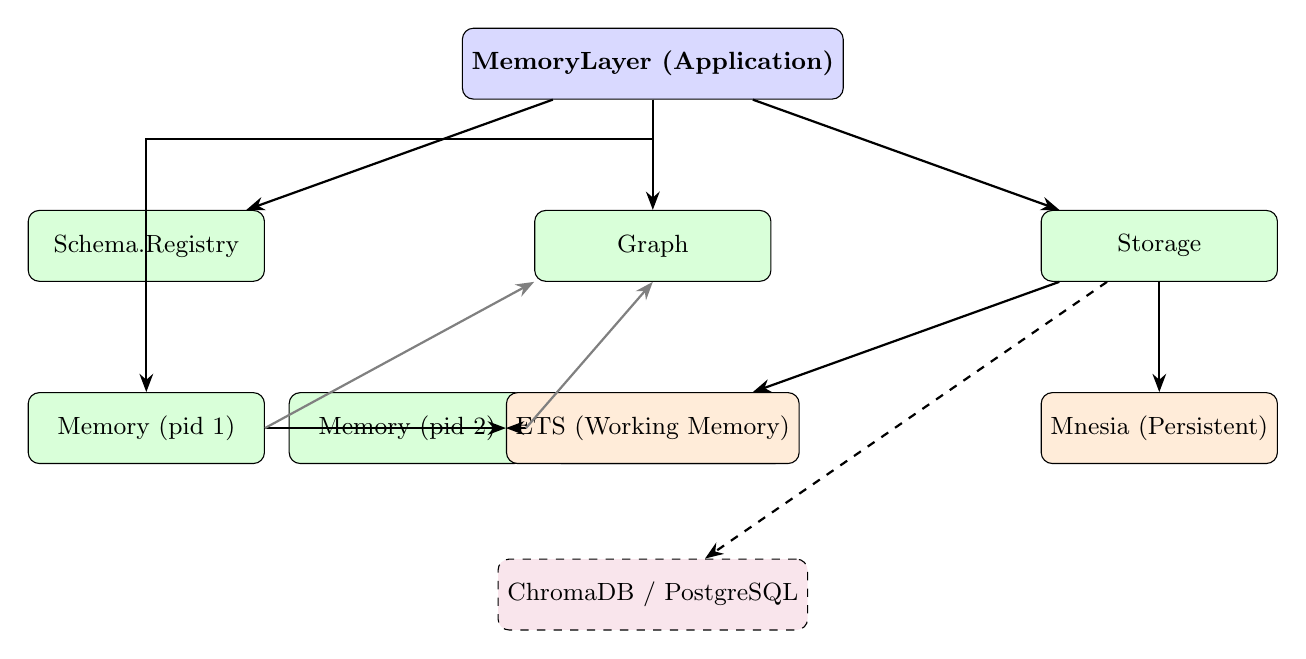
\begin{tikzpicture}[
  node distance=1.5cm and 2cm,
  every node/.style={draw, rounded corners, minimum width=3cm, minimum height=0.9cm, font=\small},
  sup/.style={fill=blue!15, font=\small\bfseries},
  gen/.style={fill=green!15},
  store/.style={fill=orange!15},
  ext/.style={fill=purple!10, dashed},
  arr/.style={-{Stealth}, thick}
]
  \node[sup] (app) {MemoryLayer (Application)};

  \node[gen, below left=1.4cm and 2.5cm of app] (schema) {Schema.Registry};
  \node[gen, below=1.4cm of app] (graph) {Graph};
  \node[gen, below right=1.4cm and 2.5cm of app] (storage) {Storage};

  \node[gen, below=1.4cm of schema] (mem1) {Memory (pid 1)};
  \node[gen, right=0.3cm of mem1] (mem2) {Memory (pid 2)};
  \node[right=0.3cm of mem2] (memn) {\ldots};

  \node[store, below=1.4cm of graph] (ets) {ETS (Working Memory)};
  \node[store, below=1.4cm of storage] (mnesia) {Mnesia (Persistent)};

  \node[ext, below=1.2cm of ets] (chroma) {ChromaDB / PostgreSQL};

  \draw[arr] (app) -- (schema);
  \draw[arr] (app) -- (graph);
  \draw[arr] (app) -- (storage);
  \draw[arr] (app.south) -- ++(0,-0.5) -| (mem1.north);

  \draw[arr] (mem1) -- (ets);
  \draw[arr] (mem2) -- (ets);
  \draw[arr] (storage) -- (ets);
  \draw[arr] (storage) -- (mnesia);
  \draw[arr, dashed] (storage) -- (chroma);

  \draw[arr, gray] (mem1.east) -- (graph.south west);
  \draw[arr, gray] (mem2.east) -- (graph.south);
\end{tikzpicture}
\caption{Memory Layer architecture.  Solid lines show OTP supervision and data flow; dashed lines show planned extensions.  Each Memory instance is a separate GenServer process.}
\label{fig:architecture}
\end{figure}

\begin{designprinciple}[Everything an agent knows is a typed memory]
Just as Plan~9 made everything a file, the memory layer makes everything a typed memory instance---facts, decisions, procedures, episodes, tasks, configurations, and even the agent's own execution traces.
\end{designprinciple}

\begin{designprinciple}[Dual-layer storage mirrors cognition]
ETS serves as working memory (fast, volatile, bounded); Mnesia serves as long-term memory (durable, queryable, unbounded).
Promotion and demotion between layers happens automatically based on access patterns.
\end{designprinciple}

\begin{designprinciple}[Per-memory process isolation]
Each memory instance runs as its own GenServer process, providing natural concurrency isolation, independent lifecycle management, and the ability to supervise individual memories.
\end{designprinciple}

The five core modules and their responsibilities:

\begin{enumerate}
  \item \textbf{\texttt{MemoryLayer.Schema}} --- Type system: 24 memory type definitions as Elixir structs, subcategory classification, and the \texttt{Registry} GenServer for runtime type resolution.
  \item \textbf{\texttt{MemoryLayer.Memory}} --- Core GenServer: per-memory stateful process with typed data, content hashing, and operations (create, wrap, data, update, evolve, merge, delete).
  \item \textbf{\texttt{MemoryLayer.Version}} --- Versioning: causal change tracking with parent-child lineage, change reason annotations, and vector clocks for multi-agent conflict detection.
  \item \textbf{\texttt{MemoryLayer.Graph}} --- Relationships: nine typed edge relations between memories, graph traversal (BFS with depth limits), neighborhood queries, and conflict detection.
  \item \textbf{\texttt{MemoryLayer.Storage}} --- Multi-backend router: fan-out writes to ETS and Mnesia, tiered recall with automatic promotion, cross-backend search, and LRU eviction.
\end{enumerate}

Table~\ref{tab:module-summary} summarizes the OTP process types:

\begin{table}[H]
\centering
\caption{OTP process types in the memory layer.}
\label{tab:module-summary}
\begin{tabularx}{\textwidth}{llX}
\toprule
\textbf{Module} & \textbf{Process Type} & \textbf{State} \\
\midrule
\texttt{MemoryLayer} & Application & Initializes ETS tables, starts Mnesia, launches supervisor \\
\texttt{Schema.Registry} & Named GenServer & Map from schema name strings to module atoms \\
\texttt{Memory} & Per-instance GenServer & Typed data struct, version, content hash, vector clock, timestamps \\
\texttt{Graph} & Named GenServer & Stateless coordinator (edges stored in Mnesia) \\
\texttt{Storage} & Named GenServer & Stateless coordinator (data in ETS + Mnesia) \\
\bottomrule
\end{tabularx}
\end{table}

% ══════════════════════════════════════════════════════════════
\section{Type System and Schema Registry}\label{sec:types}
% ══════════════════════════════════════════════════════════════

\subsection{Design Rationale}\label{subsec:type-rationale}

The fundamental design decision in the memory layer is that \emph{every memory has a type}.
Unlike traditional filesystems where a file is an opaque byte sequence, each memory instance carries a schema that defines its fields, their types, and their constraints.
This enables:

\begin{itemize}
  \item Compile-time checking via Dialyzer typespecs
  \item Runtime validation via \texttt{@enforce\_keys} and struct construction
  \item Type-safe deserialization: given a stored \texttt{schema\_name} string, the registry resolves the correct Elixir module for reconstruction
  \item Domain-specific operations: a \texttt{TodoData} memory can be queried by priority and status; a \texttt{FactData} memory can be filtered by confidence
\end{itemize}

\subsection{BaseSchema: The Universal Type}\label{subsec:base-schema}

All 24 memory types share a common envelope defined by \texttt{BaseSchema}:

\begin{lstlisting}[caption={BaseSchema: the universal memory envelope.}, label={lst:base-schema}]
defmodule MemoryLayer.Schema.BaseSchema do
  @enforce_keys [:schema_name, :content]
  defstruct [
    :schema_name,
    :content,
    :metadata,
    id: nil,
    created_at: nil,
    updated_at: nil,
    deleted_at: nil,
    content_hash: nil,
    tags: []
  ]

  @type t :: %__MODULE__{
    schema_name: String.t(),
    content: map(),
    metadata: map() | nil,
    id: String.t() | nil,
    created_at: DateTime.t() | nil,
    updated_at: DateTime.t() | nil,
    deleted_at: DateTime.t() | nil,
    content_hash: String.t() | nil,
    tags: [String.t()]
  }
end
\end{lstlisting}

The \texttt{@enforce\_keys} directive ensures that \texttt{schema\_name} and \texttt{content} must be provided at construction time---the Elixir compiler will raise an error if they are omitted.
The \texttt{deleted\_at} field supports soft deletes (Section~\ref{subsec:soft-delete}), and \texttt{content\_hash} enables deduplication (Section~\ref{subsec:content-hash}).

\subsection{The 24 Memory Types}\label{subsec:24types}

\ContextFS{} defines 24 memory types organized into six subcategories.
The classification is defined by pattern matching on the type atom:

\begin{lstlisting}[caption={Subcategory classification via pattern matching.}, label={lst:subcategory}]
defmodule MemoryLayer.Schema do
  @type memory_type ::
    :fact | :decision | :procedural | :episodic |
    :todo | :issue | :api | :schema_def |
    :workflow | :task | :step | :agent_run |
    :tag | :annotation | :embedding | :index |
    :config | :session | :context | :log |
    :person | :project | :artifact | :event

  @type subcategory ::
    :core | :extended | :workflow |
    :metadata | :system | :relational

  def subcategory(t) when t in [:fact, :decision,
    :procedural, :episodic], do: :core
  def subcategory(t) when t in [:todo, :issue,
    :api, :schema_def], do: :extended
  def subcategory(t) when t in [:workflow, :task,
    :step, :agent_run], do: :workflow
  def subcategory(t) when t in [:tag, :annotation,
    :embedding, :index], do: :metadata
  def subcategory(t) when t in [:config, :session,
    :context, :log], do: :system
  def subcategory(t) when t in [:person, :project,
    :artifact, :event], do: :relational
end
\end{lstlisting}

Table~\ref{tab:memory-types} lists all 24 types with their fields and intended use:

\begin{table}[H]
\centering
\caption{The 24 memory types in \ContextFS{}.}
\label{tab:memory-types}
\begin{tabularx}{\textwidth}{llX}
\toprule
\textbf{Subcategory} & \textbf{Type} & \textbf{Purpose and Key Fields} \\
\midrule
\multirow{4}{*}{\textbf{Core}} & \texttt{fact} & Declarative knowledge: \texttt{assertion}, \texttt{confidence}, \texttt{evidence}, \texttt{source} \\
  & \texttt{decision} & Decision records: \texttt{decision}, \texttt{rationale}, \texttt{alternatives}, \texttt{confidence} \\
  & \texttt{procedural} & How-to knowledge: \texttt{name}, \texttt{steps}, \texttt{preconditions}, \texttt{postconditions} \\
  & \texttt{episodic} & Experiential records: \texttt{event}, \texttt{outcome}, \texttt{context}, \texttt{duration\_ms} \\
\midrule
\multirow{4}{*}{\textbf{Extended}} & \texttt{todo} & Action items: \texttt{title}, \texttt{priority} (low/med/high/critical), \texttt{status} \\
  & \texttt{issue} & Problem records: \texttt{title}, \texttt{severity}, \texttt{root\_cause}, \texttt{resolution} \\
  & \texttt{api} & API schemas and access patterns \\
  & \texttt{schema\_def} & Meta-level: schemas about schemas \\
\midrule
\multirow{4}{*}{\textbf{Workflow}} & \texttt{workflow} & End-to-end processes: \texttt{name}, \texttt{steps}, \texttt{trigger}, \texttt{status} \\
  & \texttt{task} & Individual work units within workflows \\
  & \texttt{step} & Atomic operations within tasks \\
  & \texttt{agent\_run} & Execution traces: \texttt{agent\_id}, \texttt{task}, \texttt{model}, \texttt{duration\_ms}, \texttt{status} \\
\midrule
\multirow{4}{*}{\textbf{Metadata}} & \texttt{tag} & Classification labels \\
  & \texttt{annotation} & Commentary on other memories \\
  & \texttt{embedding} & Vector representations \\
  & \texttt{index} & Search index entries \\
\midrule
\multirow{4}{*}{\textbf{System}} & \texttt{config} & Configuration parameters \\
  & \texttt{session} & Agent session state \\
  & \texttt{context} & Contextual information bundles \\
  & \texttt{log} & System event records \\
\midrule
\multirow{4}{*}{\textbf{Relational}} & \texttt{person} & People known to the agent \\
  & \texttt{project} & Project-level organizational units \\
  & \texttt{artifact} & Produced outputs (documents, code, analyses) \\
  & \texttt{event} & Calendar or timeline events \\
\bottomrule
\end{tabularx}
\end{table}

\subsection{Domain Schema Definitions}\label{subsec:domain-schemas}

Each memory type is an Elixir struct with enforced keys and typespecs.
Here are three representative examples spanning the core, extended, and workflow subcategories:

\begin{lstlisting}[caption={FactData: declarative knowledge with confidence tracking.}, label={lst:fact-data}]
defmodule MemoryLayer.Schema.FactData do
  @moduledoc "Verified assertions with confidence."

  @enforce_keys [:assertion]
  defstruct [
    :assertion,
    :evidence,
    :source,
    confidence: 1.0,
    schema_name: "fact"
  ]

  @type t :: %__MODULE__{
    assertion: String.t(),
    evidence: String.t() | nil,
    source: String.t() | nil,
    confidence: float(),
    schema_name: String.t()
  }
end
\end{lstlisting}

\begin{lstlisting}[caption={IssueData: problem tracking with severity and resolution.}, label={lst:issue-data}]
defmodule MemoryLayer.Schema.IssueData do
  @enforce_keys [:title, :severity]
  defstruct [
    :title,
    :severity,
    :description,
    :resolution,
    :root_cause,
    status: :open,
    schema_name: "issue"
  ]

  @type t :: %__MODULE__{
    title: String.t(),
    severity: :low | :medium | :high | :critical,
    description: String.t() | nil,
    resolution: String.t() | nil,
    root_cause: String.t() | nil,
    status: :open | :investigating | :resolved | :closed,
    schema_name: String.t()
  }
end
\end{lstlisting}

\begin{lstlisting}[caption={AgentRunData: execution trace of an agent invocation.}, label={lst:agent-run}]
defmodule MemoryLayer.Schema.AgentRunData do
  @enforce_keys [:agent_id, :task]
  defstruct [
    :agent_id, :task, :result, :error,
    :input, :output, :duration_ms, :model,
    status: :running,
    started_at: nil,
    completed_at: nil,
    schema_name: "agent_run"
  ]

  @type t :: %__MODULE__{
    agent_id: String.t(),
    task: String.t(),
    result: term() | nil,
    error: String.t() | nil,
    input: map() | nil,
    output: map() | nil,
    duration_ms: non_neg_integer() | nil,
    model: String.t() | nil,
    status: :running | :completed | :failed | :cancelled,
    started_at: DateTime.t() | nil,
    completed_at: DateTime.t() | nil,
    schema_name: String.t()
  }
end
\end{lstlisting}

The pattern is consistent across all 24 types: \texttt{@enforce\_keys} declares the mandatory fields, \texttt{defstruct} provides defaults for optional fields, and \texttt{@type} gives the complete typespec for Dialyzer.
The \texttt{schema\_name} field is always defaulted to the type's string identifier, linking the struct to its registry entry.

\subsection{The Schema Registry}\label{subsec:registry}

The \texttt{Schema.Registry} is a GenServer that maps schema name strings to their Elixir modules, enabling type-safe deserialization at runtime:

\begin{lstlisting}[caption={Schema Registry: runtime type resolution.}, label={lst:registry}]
defmodule MemoryLayer.Schema.Registry do
  use GenServer

  @type registry_state :: %{String.t() => module()}

  def start_link(opts \\ []) do
    GenServer.start_link(__MODULE__, opts, name: __MODULE__)
  end

  @spec resolve(String.t()) ::
    {:ok, module()} | {:error, :not_found}
  def resolve(schema_name) do
    GenServer.call(__MODULE__, {:resolve, schema_name})
  end

  @spec register(String.t(), module()) :: :ok
  def register(schema_name, module) do
    GenServer.call(__MODULE__,
      {:register, schema_name, module})
  end

  @spec list() :: [String.t()]
  def list do
    GenServer.call(__MODULE__, :list)
  end

  # --- GenServer Callbacks ---

  @impl true
  def init(_opts) do
    registry = %{
      "fact"       => MemoryLayer.Schema.FactData,
      "decision"   => MemoryLayer.Schema.DecisionData,
      "procedural" => MemoryLayer.Schema.ProceduralData,
      "episodic"   => MemoryLayer.Schema.EpisodicData,
      "todo"       => MemoryLayer.Schema.TodoData,
      "issue"      => MemoryLayer.Schema.IssueData,
      "workflow"   => MemoryLayer.Schema.WorkflowData,
      "agent_run"  => MemoryLayer.Schema.AgentRunData
    }
    {:ok, registry}
  end

  @impl true
  def handle_call({:resolve, name}, _from, state) do
    case Map.fetch(state, name) do
      {:ok, module} -> {:reply, {:ok, module}, state}
      :error -> {:reply, {:error, :not_found}, state}
    end
  end

  @impl true
  def handle_call({:register, name, module}, _from, state) do
    {:reply, :ok, Map.put(state, name, module)}
  end

  @impl true
  def handle_call(:list, _from, state) do
    {:reply, Map.keys(state), state}
  end
end
\end{lstlisting}

The registry is initialized with the built-in types at application startup, and new types can be registered dynamically via \texttt{register/2}.
The mapping is injective by construction: each schema name maps to exactly one module, ensuring unambiguous type resolution.

\begin{remark}[Extensibility]
Third-party schema types can be registered at runtime without modifying the core \texttt{Schema} module.
An agent that discovers a new domain can define a struct, register it, and immediately begin creating typed memories of that new type.
\end{remark}

\subsection{Type Safety: Two Levels}\label{subsec:type-safety}

Type safety in the memory layer operates at two complementary levels:

\textbf{Compile-time (Dialyzer).}
Every public function carries an \texttt{@spec} annotation.
The Dialyzer static analysis tool traces type information through the codebase and reports mismatches.
For example, if a caller passes a \texttt{FactData} struct to a function expecting \texttt{IssueData}, Dialyzer will flag this at compile time.

\textbf{Runtime (struct enforcement).}
Elixir's \texttt{@enforce\_keys} and \texttt{defstruct} validate data at construction time.
Attempting to create a \texttt{FactData} without the required \texttt{:assertion} field raises an \texttt{ArgumentError} immediately, preventing invalid memories from entering the system.
The \texttt{is\_struct/1} guard in the Memory GenServer's \texttt{create/1} function further ensures only valid structs are accepted:

\begin{lstlisting}[caption={Guard clause ensures only structs enter the system.}, label={lst:guard}]
@spec create(struct()) :: {:ok, pid()} | {:error, term()}
def create(schema_data) when is_struct(schema_data) do
  GenServer.start_link(__MODULE__, {:create, schema_data})
end
\end{lstlisting}

% ══════════════════════════════════════════════════════════════
\section{The Memory GenServer}\label{sec:memory-genserver}
% ══════════════════════════════════════════════════════════════

\subsection{Process-Per-Memory Architecture}\label{subsec:process-per-memory}

The central design choice in the memory layer is that each memory instance is a GenServer process.
This is a natural fit for the \BEAM{}: lightweight processes are cheap (a few hundred bytes of initial memory), and the \BEAM{} scheduler handles millions of them efficiently.

Each Memory process holds the complete typed state for one memory instance:

\begin{lstlisting}[caption={Memory GenServer state type.}, label={lst:memory-state}]
defmodule MemoryLayer.Memory do
  use GenServer

  alias MemoryLayer.{Version, Storage, Graph}

  @type t :: %{
    id: String.t(),
    schema_name: String.t(),
    data: struct(),
    version: non_neg_integer(),
    content_hash: String.t(),
    vector_clock: map(),
    created_at: DateTime.t(),
    updated_at: DateTime.t(),
    deleted_at: DateTime.t() | nil
  }
\end{lstlisting}

The \texttt{data} field holds the typed schema struct (e.g., a \texttt{FactData} or \texttt{IssueData}).
The \texttt{vector\_clock} tracks causal ordering across agents (Section~\ref{sec:versioning}).
The \texttt{content\_hash} enables deduplication (Section~\ref{subsec:content-hash}).

\subsection{Creation and Initialization}\label{subsec:creation}

Creating a new memory starts a GenServer process, computes a UUID and content hash, and persists to both storage tiers:

\begin{lstlisting}[caption={Memory creation: from schema struct to supervised process.}, label={lst:memory-create}]
  @spec create(struct()) :: {:ok, pid()} | {:error, term()}
  def create(schema_data) when is_struct(schema_data) do
    GenServer.start_link(__MODULE__, {:create, schema_data})
  end

  @impl true
  def init({:create, schema_data}) do
    case build_state(schema_data) do
      {:ok, state} ->
        persist(state)
        {:ok, state}
      {:error, reason} ->
        {:stop, reason}
    end
  end

  defp build_state(schema_data, opts \\ []) do
    id = Keyword.get(opts, :id) || generate_uuid()
    now = DateTime.utc_now()

    {:ok, %{
      id: id,
      schema_name: extract_schema_name(schema_data),
      data: schema_data,
      version: 1,
      content_hash: content_hash(schema_data),
      vector_clock: %{node() => 1},
      created_at: now,
      updated_at: now,
      deleted_at: nil
    }}
  rescue
    e -> {:error, Exception.message(e)}
  end
\end{lstlisting}

Several details are worth noting:

\begin{itemize}
  \item The \texttt{vector\_clock} is initialized with the current \BEAM{} node as the sole entry, set to 1.
  In a distributed deployment, each node contributes its own clock component.
  \item The \texttt{rescue} clause catches struct validation errors (e.g., missing enforced keys) and converts them to \texttt{\{:error, reason\}} tuples, preventing the GenServer from crashing on invalid input.
  \item The \texttt{extract\_schema\_name/1} function extracts the type tag using either the struct's \texttt{schema\_name} field or, as a fallback, the module name.
\end{itemize}

\subsection{Content Hashing}\label{subsec:content-hash}

Every memory instance receives a SHA-256 content hash computed from its data:

\begin{lstlisting}[caption={Content-addressed hashing for deduplication.}, label={lst:content-hash}]
  @spec content_hash(struct()) :: String.t()
  def content_hash(data) do
    data
    |> :erlang.term_to_binary()
    |> then(&:crypto.hash(:sha256, &1))
    |> Base.encode16(case: :lower)
  end
\end{lstlisting}

This three-step pipeline---serialize, hash, encode---produces a deterministic fingerprint for any Elixir term.
Two memories with identical typed data will have the same hash regardless of when or by whom they were created.
The \texttt{update/2} handler uses this for deduplication: if the hash has not changed after applying updates, the write is skipped entirely.

\subsection{Updates with Deduplication}\label{subsec:updates}

The update handler applies changes to the underlying struct, recomputes the hash, and short-circuits if the content is unchanged:

\begin{lstlisting}[caption={Update with content-hash deduplication.}, label={lst:update}]
  @impl true
  def handle_call({:update, changes}, _from, state) do
    updated_data = struct(state.data, Map.to_list(changes))
    new_hash = content_hash(updated_data)

    if new_hash == state.content_hash do
      {:reply, :ok, state}  # No change, skip write
    else
      new_state = %{state |
        data: updated_data,
        version: state.version + 1,
        content_hash: new_hash,
        updated_at: DateTime.utc_now()
      }
      persist(new_state)
      {:reply, :ok, new_state}
    end
  end
\end{lstlisting}

The \texttt{struct/2} function applies a keyword list of changes to an existing struct, raising if any key does not exist in the struct definition.
This provides an additional layer of runtime type safety: attempting to set a nonexistent field will fail immediately.

\subsection{Evolution: Parent-Child Lineage}\label{subsec:evolution}

The \texttt{evolve/3} operation creates a new memory (child) from an existing one (parent), establishing a causal link:

\begin{lstlisting}[caption={Memory evolution with causal tracking.}, label={lst:evolve}]
  @spec evolve(pid(), map(), Version.change_reason()) ::
    {:ok, pid()} | {:error, term()}
  def evolve(pid, changes, reason) do
    GenServer.call(pid, {:evolve, changes, reason})
  end

  @impl true
  def handle_call({:evolve, changes, reason}, _from, state) do
    evolved_data = struct(state.data, Map.to_list(changes))

    case create(evolved_data) do
      {:ok, child_pid} ->
        {:ok, child_state} =
          GenServer.call(child_pid, :get_state)

        # Record version lineage in Mnesia
        Version.record(
          state.id, child_state.id,
          reason, state.vector_clock
        )

        # Establish graph edge
        Graph.link(
          state.id, child_state.id,
          :evolved_into, %{reason: reason}
        )

        {:reply, {:ok, child_pid}, state}

      {:error, reason} ->
        {:reply, {:error, reason}, state}
    end
  end
\end{lstlisting}

Evolution creates a \emph{new} process (the child) rather than mutating the parent.
This is consistent with immutable-data principles: the parent retains its original state, and the version history records the causal chain.
The operation coordinates three subsystems: Memory (creating the child process), Version (recording the lineage entry in Mnesia), and Graph (establishing an \texttt{:evolved\_into} edge).

\subsection{Merge: Conflict Resolution}\label{subsec:merge}

When two agents concurrently modify the same memory and their vector clocks are incomparable (indicating a conflict), the merge operation resolves it by creating a new memory that synthesizes both versions:

\begin{lstlisting}[caption={Merging concurrent versions with vector clock unification.}, label={lst:merge}]
  @spec merge(pid(), pid(), map()) ::
    {:ok, pid()} | {:error, term()}
  def merge(pid_a, pid_b, merged_data) do
    GenServer.call(pid_a, {:merge, pid_b, merged_data})
  end

  @impl true
  def handle_call({:merge, pid_b, merged_data},
                  _from, state_a) do
    case GenServer.call(pid_b, :get_state) do
      {:ok, state_b} ->
        case create(merged_data) do
          {:ok, merged_pid} ->
            {:ok, merged_state} =
              GenServer.call(merged_pid, :get_state)

            # Merge vector clocks: component-wise max
            merged_clock = merge_vector_clocks(
              state_a.vector_clock,
              state_b.vector_clock
            )
            GenServer.call(merged_pid,
              {:set_vector_clock, merged_clock})

            # Link both parents
            Graph.link(state_a.id, merged_state.id,
              :derived_from, %{operation: :merge})
            Graph.link(state_b.id, merged_state.id,
              :derived_from, %{operation: :merge})

            Version.record(state_a.id, merged_state.id,
              :correction, merged_clock)

            {:reply, {:ok, merged_pid}, state_a}
          {:error, reason} ->
            {:reply, {:error, reason}, state_a}
        end
      {:error, reason} ->
        {:reply, {:error, reason}, state_a}
    end
  end

  defp merge_vector_clocks(vc_a, vc_b) do
    Map.merge(vc_a, vc_b, fn _k, v1, v2 -> max(v1, v2) end)
  end
\end{lstlisting}

The merged clock takes the component-wise maximum of both parent clocks, guaranteeing that the merged version causally dominates both parents.
Both parents are linked to the child via \texttt{:derived\_from} edges, preserving the full conflict-resolution history.

\subsection{Soft Deletes}\label{subsec:soft-delete}

Memories are never physically destroyed.
The delete operation sets a \texttt{deleted\_at} timestamp (the tombstone pattern):

\begin{lstlisting}[caption={Soft delete via tombstone timestamp.}, label={lst:soft-delete}]
  @impl true
  def handle_call(:delete, _from, state) do
    new_state = %{state | deleted_at: DateTime.utc_now()}
    persist(new_state)
    {:reply, :ok, new_state}
  end

  # Data access checks for tombstone
  @impl true
  def handle_call(:get_data, _from,
    %{deleted_at: d} = state) when not is_nil(d) do
    {:reply, {:error, :deleted}, state}
  end

  def handle_call(:get_data, _from, state) do
    touch_lru(state.id)
    {:reply, {:ok, state.data}, state}
  end
\end{lstlisting}

The pattern match on \texttt{deleted\_at} in the \texttt{:get\_data} handler ensures that deleted memories return an error to callers, while the memory's graph edges and version history remain intact for lineage queries.

\subsection{Persistence: Dual-Layer Write Path}\label{subsec:persist}

Every state change is persisted to both ETS and Mnesia, with an LRU timestamp for eviction:

\begin{lstlisting}[caption={Dual-layer persistence with LRU tracking.}, label={lst:persist}]
  defp persist(state) do
    # ETS: working memory (microsecond access)
    :ets.insert(:memory_working, {state.id, state})

    # Mnesia: persistent knowledge (durable)
    Storage.save(state)

    # LRU tracking for eviction
    touch_lru(state.id)
    :ok
  end

  defp touch_lru(id) do
    :ets.insert(:memory_lru,
      {id, System.monotonic_time()})
  end
\end{lstlisting}

The \texttt{System.monotonic\_time/0} call provides a high-resolution, monotonically increasing timestamp suitable for LRU ordering.
The \texttt{:memory\_lru} ETS table is separate from \texttt{:memory\_working} to avoid coupling access metadata with memory content.

% ══════════════════════════════════════════════════════════════
\section{Versioning and Causal Tracking}\label{sec:versioning}
% ══════════════════════════════════════════════════════════════

\subsection{Change Reasons}\label{subsec:change-reasons}

Every version transition carries a \emph{change reason} explaining why the memory changed.
The four change reasons form a partial order with a subsumption relation:

\begin{lstlisting}[caption={Change reasons with subsumption ordering.}, label={lst:change-reasons}]
defmodule MemoryLayer.Version do
  @type change_reason ::
    :observation | :inference | :correction | :decay

  @spec subsumes?(change_reason(), change_reason()) ::
    boolean()
  def subsumes?(a, a), do: true
  def subsumes?(:correction, :observation), do: true
  def subsumes?(:inference, :observation), do: true
  def subsumes?(:decay, _), do: true
  def subsumes?(_, _), do: false

  @spec join_reasons(change_reason(), change_reason()) ::
    change_reason()
  def join_reasons(a, b) do
    cond do
      subsumes?(a, b) -> a
      subsumes?(b, a) -> b
      true -> :correction
    end
  end
end
\end{lstlisting}

The semantics are:
\begin{itemize}
  \item \textbf{\texttt{:observation}} --- base level: new data was directly observed.
  \item \textbf{\texttt{:inference}} --- extends observation: a conclusion derived from existing data.
  \item \textbf{\texttt{:correction}} --- subsumes observation: a previous version was wrong.
  \item \textbf{\texttt{:decay}} --- terminal: information is becoming stale or irrelevant.
\end{itemize}

The \texttt{join\_reasons/2} function computes the least upper bound when merging version histories from concurrent updates, defaulting to \texttt{:correction} when neither reason subsumes the other.

\subsection{Version Entries}\label{subsec:version-entries}

Each version entry records the full causal context of a memory change:

\begin{lstlisting}[caption={Version entry type and recording.}, label={lst:version-entry}]
  @type version_entry :: %{
    memory_id: String.t(),
    parent_id: String.t() | nil,
    version: non_neg_integer(),
    reason: change_reason(),
    vector_clock: vector_clock(),
    timestamp: DateTime.t(),
    metadata: map()
  }

  @spec record(String.t() | nil, String.t(),
    change_reason(), vector_clock()) :: :ok
  def record(parent_id, child_id, reason,
    parent_clock \\ %{}) do
    new_clock = increment_clock(parent_clock)
    version = next_version(parent_id)

    entry = %{
      memory_id: child_id,
      parent_id: parent_id,
      version: version,
      reason: reason,
      vector_clock: new_clock,
      timestamp: DateTime.utc_now(),
      metadata: %{}
    }

    {:atomic, :ok} =
      :mnesia.transaction(fn ->
        :mnesia.write({:versions, child_id, entry})
        :ok
      end)
    :ok
  end
\end{lstlisting}

Version entries are stored in the Mnesia \texttt{:versions} table using the bag table type, which allows multiple entries per key.
This enables the complete version history for a memory to be retrieved in a single query.
The Mnesia transaction wrapper ensures atomicity: the version entry is either fully written or not at all.

\subsection{History and Lineage Traversal}\label{subsec:history}

Two query functions provide different views of version history:

\begin{lstlisting}[caption={Version history and lineage chain traversal.}, label={lst:history}]
  @spec history(String.t()) :: [version_entry()]
  def history(memory_id) do
    {:atomic, entries} =
      :mnesia.transaction(fn ->
        :mnesia.match_object(
          {:versions, memory_id, :_})
      end)

    entries
    |> Enum.map(fn {:versions, _id, entry} -> entry end)
    |> Enum.sort_by(& &1.timestamp, DateTime)
  end

  @spec lineage(String.t()) :: [version_entry()]
  def lineage(memory_id) do
    case history(memory_id) do
      [] -> []
      [entry | _] = entries ->
        case entry.parent_id do
          nil -> entries
          parent_id -> lineage(parent_id) ++ entries
        end
    end
  end
\end{lstlisting}

The \texttt{history/1} function returns all version entries for a single memory, sorted by timestamp.
The \texttt{lineage/1} function follows the \texttt{parent\_id} chain recursively back to the root, building the complete causal path.

\subsection{Vector Clocks}\label{subsec:vector-clocks}

In multi-agent settings, memories may be updated concurrently by different agents.
Vector clocks~\citep{lamport1978time, fidge1988timestamps} establish causal ordering.
Each agent maintains a counter; on write, the writing agent increments its component.

\begin{lstlisting}[caption={Vector clock comparison for conflict detection.}, label={lst:vector-clocks}]
  @type vector_clock ::
    %{optional(atom() | String.t()) => non_neg_integer()}
  @type clock_ordering ::
    :before | :after | :concurrent | :equal

  @spec compare_clocks(vector_clock(), vector_clock()) ::
    clock_ordering()
  def compare_clocks(vc_a, vc_b) when vc_a == vc_b,
    do: :equal

  def compare_clocks(vc_a, vc_b) do
    all_keys = Map.keys(vc_a) ++ Map.keys(vc_b)
      |> Enum.uniq()

    comparisons = Enum.map(all_keys, fn key ->
      a_val = Map.get(vc_a, key, 0)
      b_val = Map.get(vc_b, key, 0)
      cond do
        a_val < b_val -> :less
        a_val > b_val -> :greater
        true -> :equal
      end
    end)

    has_less = :less in comparisons
    has_greater = :greater in comparisons

    cond do
      has_less and has_greater -> :concurrent
      has_less -> :before
      has_greater -> :after
      true -> :equal
    end
  end

  @spec increment_clock(vector_clock()) :: vector_clock()
  def increment_clock(vc) do
    Map.update(vc, node(), 1, &(&1 + 1))
  end

  @spec merge_clocks(vector_clock(), vector_clock()) ::
    vector_clock()
  def merge_clocks(vc_a, vc_b) do
    Map.merge(vc_a, vc_b,
      fn _key, v1, v2 -> max(v1, v2) end)
  end
\end{lstlisting}

Two clocks are \emph{concurrent} when neither dominates the other (one has a strictly greater component for some agent while the other is strictly greater for a different agent).
Concurrent clocks signal a conflict requiring explicit resolution through the merge operation (Section~\ref{subsec:merge}).

The vector clock operations are pure functions over immutable maps, making them safe for concurrent use and easy to reason about.

% ══════════════════════════════════════════════════════════════
\section{Graph Relationships}\label{sec:graph}
% ══════════════════════════════════════════════════════════════

\subsection{Edge Relations}\label{subsec:edge-relations}

The memory graph captures typed relationships between memory instances.
Nine edge relations define the vocabulary of relationships:

\begin{lstlisting}[caption={The nine edge relation types.}, label={lst:edge-relations}]
defmodule MemoryLayer.Graph do
  use GenServer

  @type edge_relation ::
    :evolved_into  | :references   | :supersedes |
    :contradicts   | :supports     | :derived_from |
    :part_of       | :triggers     | :blocked_by

  @type edge :: %{
    from: String.t(),
    to: String.t(),
    relation: edge_relation(),
    metadata: map(),
    created_at: DateTime.t()
  }
\end{lstlisting}

Table~\ref{tab:edge-relations} describes the semantics of each edge type:

\begin{table}[H]
\centering
\caption{Edge relation semantics.}
\label{tab:edge-relations}
\begin{tabularx}{\textwidth}{lX}
\toprule
\textbf{Relation} & \textbf{Semantics} \\
\midrule
\texttt{evolved\_into} & Memory evolved into a new version (set by \texttt{evolve/3}) \\
\texttt{references} & Memory refers to another for context \\
\texttt{supersedes} & Memory replaces an older, outdated one \\
\texttt{contradicts} & Memory conflicts with another (triggers conflict resolution) \\
\texttt{supports} & Memory provides evidence for another \\
\texttt{derived\_from} & Memory was derived from one or more parents (set by \texttt{merge/3}) \\
\texttt{part\_of} & Memory is a component of a larger memory \\
\texttt{triggers} & Memory causes creation of another \\
\texttt{blocked\_by} & Memory cannot proceed until another is resolved \\
\bottomrule
\end{tabularx}
\end{table}

\subsection{Link and Unlink}\label{subsec:link-unlink}

Edges are stored in the Mnesia \texttt{:edges} table with a composite key \texttt{\{from\_id, to\_id\}}:

\begin{lstlisting}[caption={Creating and soft-removing graph edges.}, label={lst:link-unlink}]
  @spec link(String.t(), String.t(), edge_relation(),
    map()) :: :ok | {:error, term()}
  def link(from_id, to_id, relation, metadata \\ %{}) do
    GenServer.call(__MODULE__,
      {:link, from_id, to_id, relation, metadata})
  end

  @impl true
  def handle_call({:link, from_id, to_id, relation,
    metadata}, _from, state) do
    edge = %{
      from: from_id, to: to_id,
      relation: relation, metadata: metadata,
      created_at: DateTime.utc_now()
    }
    result = :mnesia.transaction(fn ->
      :mnesia.write({:edges, {from_id, to_id}, edge})
    end)
    case result do
      {:atomic, _} -> {:reply, :ok, state}
      {:aborted, reason} -> {:reply, {:error, reason}, state}
    end
  end
\end{lstlisting}

The \texttt{unlink/3} operation follows the same tombstone pattern as memory deletion: rather than physically removing the edge, it adds a \texttt{deleted\_at} timestamp to the edge metadata.
Query functions filter out tombstoned edges.

\subsection{Graph Traversal}\label{subsec:graph-traversal}

The graph module provides breadth-first traversal with configurable depth, direction, and relation filters:

\begin{lstlisting}[caption={BFS graph traversal with depth limiting.}, label={lst:graph-traverse}]
  @type traverse_opts :: [
    max_depth: non_neg_integer(),
    direction: :forward | :reverse | :both,
    filter_relations: [edge_relation()]
  ]

  @spec traverse(String.t(), [edge_relation()],
    traverse_opts()) :: [String.t()]
  def traverse(start_id, pattern, opts \\ []) do
    GenServer.call(__MODULE__,
      {:traverse, start_id, pattern, opts})
  end

  # Private BFS implementation
  defp do_traverse(_, _, _, 0, visited), do: visited
  defp do_traverse([], _, _, _, visited), do: visited

  defp do_traverse(frontier, relations, direction,
    depth, visited) do
    new_visited = Enum.reduce(frontier, visited,
      &MapSet.put(&2, &1))

    next_frontier =
      Enum.flat_map(frontier, fn node_id ->
        edges = case direction do
          :forward -> do_edges_from(node_id)
          :reverse -> do_edges_to(node_id)
          :both ->
            do_edges_from(node_id) ++
            do_edges_to(node_id)
        end

        edges
        |> Enum.filter(& &1.relation in relations)
        |> Enum.map(fn edge ->
          case direction do
            :forward -> edge.to
            :reverse -> edge.from
            :both ->
              if edge.from == node_id,
                do: edge.to, else: edge.from
          end
        end)
        |> Enum.reject(&MapSet.member?(new_visited, &1))
      end)
      |> Enum.uniq()

    do_traverse(next_frontier, relations, direction,
      depth - 1, new_visited)
  end
\end{lstlisting}

The traversal uses a \texttt{MapSet} to track visited nodes, preventing cycles in the graph from causing infinite loops.
The pattern parameter specifies which edge relations to follow, enabling targeted queries like ``find all memories this one evolved into'' or ``find the full derivation chain''.

\subsection{Neighborhood Queries}\label{subsec:neighborhood}

The \texttt{neighborhood/2} function returns all memories connected to a given memory within a depth limit, along with their connecting edges:

\begin{lstlisting}[caption={Neighborhood query: local subgraph extraction.}, label={lst:neighborhood}]
  @spec neighborhood(String.t(), non_neg_integer()) ::
    [{String.t(), edge()}]
  def neighborhood(memory_id, max_depth \\ 2) do
    GenServer.call(__MODULE__,
      {:neighborhood, memory_id, max_depth})
  end
\end{lstlisting}

This is useful for building context around a memory: given a fact, the neighborhood reveals its supporting evidence, contradicting claims, derived decisions, and related tasks.

\subsection{Conflict Detection}\label{subsec:conflict-detection}

The graph module provides a convenience function for finding unresolved conflicts:

\begin{lstlisting}[caption={Detecting unresolved conflicts via contradicts edges.}, label={lst:conflicts}]
  @spec conflicts(String.t()) :: [{String.t(), String.t()}]
  def conflicts(memory_id) do
    edges_of_type(memory_id, :contradicts)
    |> Enum.map(fn edge -> {edge.from, edge.to} end)
  end
\end{lstlisting}

When vector clocks detect concurrent modifications, the system creates \texttt{:contradicts} edges.
Agents or operators can query for unresolved conflicts and apply the merge operation to resolve them.

% ══════════════════════════════════════════════════════════════
\section{Multi-Backend Storage Router}\label{sec:storage}
% ══════════════════════════════════════════════════════════════

\subsection{The StorageBackend Behaviour}\label{subsec:storage-behaviour}

The storage subsystem is built on an Elixir \emph{behaviour}---the functional equivalent of an interface or protocol.
Any module that implements these five callbacks can serve as a storage backend:

\begin{lstlisting}[caption={StorageBackend behaviour: the five required callbacks.}, label={lst:storage-behaviour}]
defmodule MemoryLayer.StorageBackend do
  @callback save(memory :: map()) ::
    :ok | {:error, term()}
  @callback recall(id :: String.t()) ::
    {:ok, map()} | {:error, :not_found}
  @callback search(query :: String.t(), opts :: keyword()) ::
    {:ok, [map()]} | {:error, term()}
  @callback delete(id :: String.t()) ::
    :ok | {:error, term()}
  @callback update(memory :: map()) ::
    :ok | {:error, term()}
end
\end{lstlisting}

This behaviour establishes a contract that all backends must fulfill.
The Elixir compiler warns if a module declares \texttt{@behaviour MemoryLayer.StorageBackend} but fails to implement all callbacks.

\subsection{The Storage Router}\label{subsec:storage-router}

The \texttt{Storage} module implements the \texttt{StorageBackend} behaviour itself, acting as a router that coordinates ETS and Mnesia:

\begin{lstlisting}[caption={Storage router: fan-out save to ETS and Mnesia.}, label={lst:storage-save}]
defmodule MemoryLayer.Storage do
  use GenServer
  @behaviour MemoryLayer.StorageBackend

  # Fan-out save: write to both backends
  @impl MemoryLayer.StorageBackend
  def save(memory) do
    # ETS: fast working memory
    :ets.insert(:memory_working, {memory.id, memory})

    # Mnesia: durable persistent storage
    result = :mnesia.transaction(fn ->
      :mnesia.write({:memories, memory.id, memory})
    end)

    case result do
      {:atomic, _} -> :ok
      {:aborted, reason} -> {:error, reason}
    end
  end
\end{lstlisting}

\subsection{Tiered Recall with Automatic Promotion}\label{subsec:tiered-recall}

The recall path checks ETS first (microsecond latency) and falls back to Mnesia (millisecond latency), automatically promoting Mnesia-only memories into ETS for subsequent fast access:

\begin{lstlisting}[caption={Tiered recall: ETS fast path with Mnesia fallback and promotion.}, label={lst:storage-recall}]
  @impl MemoryLayer.StorageBackend
  def recall(id) do
    case recall_from_ets(id) do
      {:ok, memory} ->
        {:ok, memory}
      {:error, :not_found} ->
        case recall_from_mnesia(id) do
          {:ok, memory} ->
            # Promote to ETS for fast future access
            :ets.insert(:memory_working, {id, memory})
            {:ok, memory}
          error ->
            error
        end
    end
  end

  defp recall_from_ets(id) do
    case :ets.lookup(:memory_working, id) do
      [{^id, memory}] -> {:ok, memory}
      [] -> {:error, :not_found}
    end
  end

  defp recall_from_mnesia(id) do
    result = :mnesia.transaction(fn ->
      :mnesia.read({:memories, id})
    end)
    case result do
      {:atomic, [{:memories, ^id, memory}]} ->
        {:ok, memory}
      {:atomic, []} ->
        {:error, :not_found}
      {:aborted, reason} ->
        {:error, reason}
    end
  end
\end{lstlisting}

Note the use of the pin operator (\texttt{\^{}id}) in the pattern matches to ensure the recalled memory's ID matches the requested one.

\subsection{Cross-Backend Search}\label{subsec:cross-backend-search}

The search function dispatches to different backends based on the query type:

\begin{lstlisting}[caption={Multi-backend search dispatch.}, label={lst:storage-search}]
  @impl MemoryLayer.StorageBackend
  def search(query, opts \\ []) do
    backend = Keyword.get(opts, :backend, :all)
    limit = Keyword.get(opts, :limit, 50)
    include_deleted = Keyword.get(opts, :include_deleted, false)
    filter = Keyword.get(opts, :filter, %{})

    results = case backend do
      :ets      -> search_ets(query, filter)
      :exact    -> search_mnesia(query, filter)
      :mnesia   -> search_mnesia(query, filter)
      :semantic -> search_mnesia(query, filter)
      :graph    -> search_mnesia(query, filter)
      :all      -> merge_search_results([
                     search_ets(query, filter),
                     search_mnesia(query, filter)
                   ])
    end

    filtered = results
      |> maybe_exclude_deleted(include_deleted)
      |> Enum.take(limit)

    {:ok, filtered}
  end
\end{lstlisting}

The \texttt{:semantic} and \texttt{:graph} backends currently fall back to Mnesia search; they are extension points for future backends (ChromaDB for vector search, FalkorDB for graph traversal).
When dispatching to \texttt{:all}, results from both backends are merged with deduplication by memory ID.

\subsection{Text Matching and Filtering}\label{subsec:text-matching}

The search pipeline applies structural filtering (matching map fields) and text matching (substring search across the serialized memory):

\begin{lstlisting}[caption={Filter and text-match pipeline.}, label={lst:filter-pipeline}]
  defp apply_filter(memories, filter) when filter == %{},
    do: memories

  defp apply_filter(memories, filter) do
    Enum.filter(memories, fn memory ->
      Enum.all?(filter, fn {key, value} ->
        Map.get(memory, key) == value
      end)
    end)
  end

  defp apply_text_match(memories, ""), do: memories

  defp apply_text_match(memories, query) do
    query_lower = String.downcase(query)
    Enum.filter(memories, fn memory ->
      memory
      |> inspect()
      |> String.downcase()
      |> String.contains?(query_lower)
    end)
  end
\end{lstlisting}

The filter pipeline demonstrates Elixir's pattern matching on function heads: the empty-filter and empty-query cases are handled by dedicated function clauses that short-circuit the processing.

\subsection{LRU Eviction}\label{subsec:lru-eviction}

Working memory (ETS) is bounded.
The eviction function demotes least-recently-used memories to Mnesia-only storage:

\begin{lstlisting}[caption={LRU eviction from working memory.}, label={lst:eviction}]
  @spec evict_lru(non_neg_integer()) :: non_neg_integer()
  def evict_lru(keep \\ 1000) do
    current_size = :ets.info(:memory_working, :size)

    if current_size > keep do
      lru_entries = :ets.tab2list(:memory_lru)
        |> Enum.sort_by(fn {_id, time} -> time end)

      to_evict = Enum.take(lru_entries,
        current_size - keep)

      Enum.each(to_evict, fn {id, _time} ->
        :ets.delete(:memory_working, id)
        :ets.delete(:memory_lru, id)
      end)

      length(to_evict)
    else
      0
    end
  end
\end{lstlisting}

Evicted memories are not lost---they remain in Mnesia and will be promoted back to ETS on the next recall.
This creates a natural working-set behavior: frequently accessed memories stay in fast storage, while rarely accessed memories settle into durable-only storage.

\subsection{Working Memory vs.\ Persistent Knowledge}\label{subsec:working-vs-persistent}

The dual-layer architecture mirrors human cognitive architecture:

\begin{table}[H]
\centering
\caption{Storage tier comparison.}
\label{tab:storage-tiers}
\begin{tabularx}{\textwidth}{lXX}
\toprule
\textbf{Property} & \textbf{ETS (Working Memory)} & \textbf{Mnesia (Persistent Knowledge)} \\
\midrule
Latency & Microseconds & Milliseconds \\
Durability & Volatile (lost on crash) & Durable (disk-backed) \\
Capacity & Bounded (LRU eviction) & Unbounded \\
Access & In-process, concurrent reads & Transactional, distributed \\
Analogy & Working memory~\citep{baddeley1992working} & Long-term memory \\
\bottomrule
\end{tabularx}
\end{table}

The promotion/demotion protocol:
\begin{enumerate}
  \item \textbf{Create}: written to both ETS and Mnesia (fan-out).
  \item \textbf{Recall}: if in ETS, return immediately; if only in Mnesia, load into ETS (promotion).
  \item \textbf{Evict}: remove from ETS, retain in Mnesia (demotion).
  \item \textbf{Bound}: LRU eviction triggers when ETS size exceeds threshold.
\end{enumerate}

% ══════════════════════════════════════════════════════════════
\section{Reliability Guarantees}\label{sec:reliability}
% ══════════════════════════════════════════════════════════════

\subsection{ACID Properties via Mnesia Transactions}\label{subsec:acid}

All Mnesia operations in the memory layer are wrapped in transactions:

\begin{enumerate}
  \item \textbf{Atomicity}: Mnesia transactions are all-or-nothing; a failed write rolls back all changes within the transaction.
  \item \textbf{Consistency}: schema validation via struct enforcement and typespecs ensures that only valid memory instances are persisted.
  \item \textbf{Isolation}: Mnesia's transaction manager serializes concurrent writes to the same memory.
  \item \textbf{Durability}: Mnesia's \texttt{disc\_copies} table type writes to both RAM and disk, surviving node restarts.
\end{enumerate}

\subsection{Type Preservation Under Round-Trip}\label{subsec:round-trip}

\begin{theorem}[Round-Trip Type Preservation]\label{thm:round-trip}
For any schema type $S$ and memory instance $m$ of type $S$: if $m$ is saved to storage and subsequently recalled, the recalled data is type-equivalent to $m$.
That is, \texttt{recall(save(m)).data} reconstructs a struct of the same type with identical field values.
\end{theorem}

\begin{proof}[Proof sketch]
The save path serializes the Elixir term (including struct metadata) via \texttt{:erlang.term\_to\_binary/1} when stored in Mnesia, or stores the term directly in ETS.
The recall path retrieves the exact term.
Since Elixir structs carry their module name as part of the term representation, and ETS/Mnesia preserve Erlang terms exactly, the recalled value is identical to the stored value.
The \texttt{schema\_name} field provides a secondary check: the Schema Registry resolves it to the correct module, confirming type consistency.
\end{proof}

\subsection{Deduplication Soundness}\label{subsec:dedup-soundness}

\begin{proposition}[Deduplication Soundness]\label{prop:dedup}
Content hashing is sound for deduplication: if $h(m_1) = h(m_2)$, then $m_1.\mathtt{data} = m_2.\mathtt{data}$ with overwhelming probability ($1 - 2^{-256}$).
\end{proposition}

The SHA-256 hash is computed over the canonical binary serialization of the data struct.
The \texttt{:erlang.term\_to\_binary/1} function produces a deterministic encoding for any Elixir term, ensuring that structurally identical data always produces the same hash.

\subsection{Conflict Detection Completeness}\label{subsec:conflict-completeness}

\begin{proposition}[Conflict Detection]\label{prop:conflict}
Vector clock comparison detects all concurrent modifications.
If two agents independently modify a memory without observing each other's changes, their resulting vector clocks will be incomparable, and \texttt{compare\_clocks/2} will return \texttt{:concurrent}.
\end{proposition}

This follows directly from the properties of vector clocks~\citep{fidge1988timestamps}: the comparison returns \texttt{:concurrent} exactly when neither clock component-wise dominates the other, which occurs precisely when the modifications are causally independent.

\subsection{Soft Delete Lineage Preservation}\label{subsec:lineage-preservation}

\begin{proposition}[Lineage Preservation]
Soft deletion preserves the complete graph structure.
All edges incident to a deleted memory remain in the Mnesia \texttt{:edges} table, and lineage queries (\texttt{Version.lineage/1}, \texttt{Graph.traverse/3}) can still traverse through deleted nodes.
\end{proposition}

This is essential for maintaining an accurate history: even when a fact is retracted (soft-deleted), the chain of reasoning that led to it---and the corrections that followed---remains queryable.

% ══════════════════════════════════════════════════════════════
\section{MCP Server Interface}\label{sec:mcp}
% ══════════════════════════════════════════════════════════════

\ContextFS{} exposes memory operations via the Model Context Protocol (MCP)~\citep{anthropic2024mcp}, enabling any MCP-compatible client (Claude, GPT, custom agents) to access the memory layer.
The MCP server translates tool calls into GenServer messages, ensuring that all access goes through the typed memory interface.

\begin{table}[H]
\centering
\caption{MCP tools exposed by \ContextFS{}.}
\label{tab:mcp-tools}
\begin{tabularx}{\textwidth}{lX}
\toprule
\textbf{Tool} & \textbf{Description} \\
\midrule
\texttt{contextfs\_save} & Create and persist a new typed memory \\
\texttt{contextfs\_recall} & Retrieve a memory by ID with full type reconstruction \\
\texttt{contextfs\_search} & Multi-backend search (exact, semantic, graph) \\
\texttt{contextfs\_evolve} & Create a new version linked to parent with change reason \\
\texttt{contextfs\_link} & Establish a typed edge between two memories \\
\texttt{contextfs\_delete} & Soft-delete (tombstone) a memory \\
\texttt{contextfs\_update} & Update fields of an existing memory \\
\texttt{contextfs\_list} & List memories by type, tag, or time range \\
\texttt{contextfs\_index} & Trigger re-indexing of embedding vectors \\
\texttt{contextfs\_sync} & Synchronize local and cloud backends \\
\bottomrule
\end{tabularx}
\end{table}

An example MCP tool call:

\begin{lstlisting}[style=jsonstyle, caption={MCP tool call for saving a typed memory.}, label={lst:mcp-example}]
{
  "jsonrpc": "2.0",
  "method": "tools/call",
  "params": {
    "name": "contextfs_save",
    "arguments": {
      "content": "Login test requires 60s timeout",
      "memory_type": "fact",
      "metadata": {
        "confidence": 0.95,
        "source": "test_run_2026_03_10"
      },
      "tags": ["testing", "timeout", "login"]
    }
  },
  "id": 42
}
\end{lstlisting}

The MCP server receives this JSON-RPC message, constructs a \texttt{FactData} struct from the arguments, calls \texttt{Memory.create/1}, and returns the resulting memory ID and metadata to the client.

% ══════════════════════════════════════════════════════════════
\section{Case Studies}\label{sec:case-studies}
% ══════════════════════════════════════════════════════════════

\subsection{Agent Learning from Past Executions}\label{subsec:case-learning}

Consider a testing agent that executes web application tests across multiple sessions.
Without persistent memory, each session starts with no knowledge of past failures.
With the memory layer:

\begin{enumerate}
  \item After each test run, the agent creates \texttt{episodic} memories recording what was tested, what failed, and what succeeded.
  \item Failed test patterns are stored as \texttt{fact} memories with confidence scores and suspected causes.
  \item When the agent encounters a similar failure in a subsequent session, search retrieves relevant past episodes, and the agent applies learned strategies.
  \item Over time, \texttt{procedural} memories accumulate: ``When test X fails with error Y, the root cause is usually Z.''
\end{enumerate}

The version lineage tracks how the agent's understanding evolves:

\begin{lstlisting}[caption={Agent learning: recording and evolving from test failures.}, label={lst:case-learning}]
# Session N: Agent encounters a test failure
{:ok, episode} = Memory.create(%EpisodicData{
  event: "login_test_timeout",
  context: %{url: "https://app.example.com/login"},
  outcome: :failure,
  duration_ms: 30_000
})

# Search for similar past failures
{:ok, similar} = Storage.search(
  "login test timeout failure",
  backend: :all, limit: 5
)

# Found a previous procedural fix -- apply and record
{:ok, _evolved} = Memory.evolve(episode, %{
  outcome: :success,
  context: %{
    url: "https://app.example.com/login",
    resolution: "Increased timeout to 60s per PROC-442"
  }
}, :correction)
\end{lstlisting}

\subsection{Cross-Session Continuity}\label{subsec:case-continuity}

A software engineering agent works on a multi-day project.
Between sessions, the user may make changes that invalidate the agent's assumptions:

\begin{lstlisting}[caption={Cross-session context restoration and assumption checking.}, label={lst:case-continuity}]
# Session start: recall last session state
{:ok, sessions} = Storage.search("",
  backend: :exact,
  filter: %{schema_name: "session"},
  limit: 1
)
last_session = hd(sessions)

# Recall all in-progress TODOs
{:ok, todos} = Storage.search("",
  backend: :exact,
  filter: %{schema_name: "todo"}
)

# Check for invalidated assumptions
for todo <- todos do
  deps = Graph.traverse(todo.id, [:references],
    max_depth: 2)
  for dep_id <- deps do
    {:ok, dep} = Storage.recall(dep_id)
    if stale?(dep) do
      # Evolve the stale fact with correction reason
      Memory.evolve(dep.id, %{
        confidence: 0.3
      }, :decay)
    end
  end
end
\end{lstlisting}

The graph lineage preserves the full narrative: original plan, partial execution, external change, plan revision.

\subsection{Multi-Agent Shared Knowledge Base}\label{subsec:case-multi-agent}

Multiple agents collaborate on a shared codebase, each responsible for different modules:

\begin{enumerate}
  \item Agent~A (frontend) discovers a bug and creates an \texttt{issue} memory.
  \item Agent~B (backend) receives the issue via Mnesia replication.
  \item Agent~B investigates and creates a \texttt{decision} memory linked to the issue via \texttt{:derived\_from}.
  \item Agent~A detects the decision via graph traversal and creates \texttt{task} memories linked via \texttt{:triggers}.
\end{enumerate}

Vector clocks detect concurrent edits:

\begin{lstlisting}[caption={Multi-agent conflict detection via vector clocks.}, label={lst:case-multi}]
# Agent A writes with its clock component
vc_a = %{agent_a: 5, agent_b: 3}

# Agent B writes concurrently
vc_b = %{agent_a: 4, agent_b: 4}

# Neither dominates: conflict detected
case Version.compare_clocks(vc_a, vc_b) do
  :concurrent ->
    # Flag for merge resolution
    Graph.link(mem_a_id, mem_b_id, :contradicts,
      %{resolution: :pending})

    # Resolve by merging
    {:ok, _merged} = Memory.merge(
      mem_a_pid, mem_b_pid,
      reconciled_data
    )
  :before -> :ok
  :after  -> :ok
end
\end{lstlisting}

% ══════════════════════════════════════════════════════════════
\section{Discussion}\label{sec:discussion}
% ══════════════════════════════════════════════════════════════

\subsection{Comparison to Unix VFS}\label{subsec:unix-vfs}

The Unix Virtual Filesystem Switch and our Storage router share the goal of providing a uniform interface over heterogeneous storage backends.
However, the VFS operates at the byte-stream level: \texttt{read(fd, buf, count)} makes no type promises about the bytes returned.
Our Storage router operates at the typed-schema level: \texttt{recall(id)} returns a memory with compile-time and runtime type guarantees.

The VFS uses inodes as the unit of storage; we use typed memory instances.
The VFS organizes files in a tree hierarchy; we organize memories in a labeled graph.
The VFS supports a fixed set of operations; our \texttt{StorageBackend} behaviour supports extensible operation sets.

\subsection{Comparison to Plan 9}\label{subsec:plan9}

Plan~9's insight was that \emph{everything should be a file}.
Our analogous principle is that \emph{everything an agent knows should be a typed memory}---including execution traces (\texttt{agent\_run}), task queues (\texttt{todo}), and configuration (\texttt{config}).

Plan~9 used synthetic file servers to present dynamic state as files.
We use MCP tools to present dynamic memory state as structured, queryable knowledge.
The key advance is that our ``files'' carry schemas, versions, and graph relationships.

\subsection{Comparison to Knowledge Graphs}\label{subsec:kg-comparison}

Knowledge graphs (Wikidata, Neo4j) store entities and relationships but typically lack:
\begin{itemize}
  \item \textbf{Schema-indexed typing}: KG nodes are loosely typed with optional properties.
  Our structs enforce strict schemas with compile-time and runtime checking.
  \item \textbf{Causal versioning}: KGs store current state; versioning is external.
  Our Version module integrates versioning as a first-class concern with causal annotations.
  \item \textbf{Multi-modal storage}: KGs and vector stores are typically separate systems.
  Our Storage router unifies them behind a single behaviour.
\end{itemize}

\subsection{Relation to Cognitive Architectures}\label{subsec:cognitive}

Soar~\citep{laird2012soar} distinguished working memory, long-term declarative, procedural, and episodic memory---a taxonomy our 24 types refine and extend.
ACT-R~\citep{anderson2004actr} formalized memory retrieval as activation-based competition, which inspired our LRU-based promotion/demotion between ETS and Mnesia.
Generative agents~\citep{park2023generative} demonstrated that LLM agents benefit from structured memory stores, though their implementation lacked type safety and formal versioning.

\subsection{Connections to Category Theory}\label{subsec:cat-connections}

For readers familiar with category theory, the design has natural categorical interpretations:

\begin{itemize}
  \item The \textbf{Schema module} defines a category whose objects are the 24 typed schemas and whose morphisms are schema transformations (field projections, type coercions).
  The \texttt{BaseSchema} is an initial object.
  \item The \textbf{Storage router} is a coproduct of storage backends: it exposes the union of all backend capabilities through injection morphisms.
  \item The \textbf{Memory GenServer} acts as a functor from the schema category to a storage category, mapping each schema type to its storage representation while preserving type structure.
  \item The \textbf{evolve/merge/split operations} form a monad on the category of memory instances: evolve is the unit (embedding a memory into a ``pending change'' context), merge is the multiplication (flattening nested changes), and the monad laws correspond to associativity and identity of operation composition.
  \item \textbf{Version tracking} is a functor from a timeline category (a thin category where objects are timestamps and morphisms are temporal orderings) to the storage category.
  \item The \textbf{graph relationships} exhibit 2-categorical structure: edges are 1-morphisms between memories, and equivalences between different edge paths (e.g., ``evolved\_into'' vs.\ ``supersedes'') are 2-morphisms.
\end{itemize}

These connections are not decorative---they explain \emph{why} the design composes cleanly.
The functor laws guarantee that type structure is preserved across storage round-trips.
The monad laws guarantee that chained evolutions and merges produce consistent results regardless of grouping.
The coproduct construction guarantees that adding a new storage backend preserves all existing capabilities.

\subsection{Relation to Version Control}\label{subsec:vcs}

Git~\citep{chacon2014pro} uses content-addressable storage with a DAG of commits.
Our version lineage is analogous but operates on typed memory instances rather than file trees.
Our change reasons provide semantic annotations that Git commit messages cannot enforce structurally.
Our vector clocks provide causal ordering in distributed settings, whereas Git relies on a total ordering of commits within each branch.

\subsection{Limitations and Future Work}\label{subsec:limitations}

Several limitations merit future investigation:

\begin{enumerate}
  \item \textbf{Garbage collection}: the tombstone pattern means storage grows monotonically.
  A formal garbage collection policy (analogous to generational GC) would bound storage while preserving essential lineage.
  \item \textbf{Schema migration}: when a schema's definition changes (fields added or removed), existing memories must be migrated.
  The framework handles this through schema transformations, but the migration strategy needs automation.
  \item \textbf{Scalability}: Mnesia's distribution model has known limitations beyond a few hundred nodes.
  For planetary-scale deployments, a CockroachDB or FoundationDB backend would be needed.
  \item \textbf{Embedding drift}: as embedding models are updated, previously computed vectors may become inconsistent.
  Re-indexing strategies need formal treatment.
  \item \textbf{Privacy and forgetting}: the ``right to be forgotten'' conflicts with the tombstone pattern.
  A cryptographic erasure scheme would reconcile these requirements.
  \item \textbf{Vector search backend}: the current implementation stubs out semantic search.
  A ChromaDB or Qdrant backend implementing the \texttt{StorageBackend} behaviour would complete the multi-modal search capability.
  \item \textbf{Graph database backend}: similarly, a FalkorDB or Neo4j backend would enable more efficient graph traversal than the current Mnesia-based BFS.
\end{enumerate}

% ══════════════════════════════════════════════════════════════
\section{Related Work}\label{sec:related}
% ══════════════════════════════════════════════════════════════

\textbf{Agent architectures with memory.}
Soar~\citep{laird2012soar} and ACT-R~\citep{anderson2004actr} established the cognitive architecture paradigm with distinct memory systems.
MemGPT~\citep{packer2023memgpt} introduced OS-inspired memory tiers for LLMs, with a main context (working memory) and external storage (archival memory).
Our framework provides stronger type guarantees and richer relationship structure than MemGPT.
Generative agents~\citep{park2023generative} demonstrated the value of structured memory for believable agent behavior but used ad-hoc storage without formal typing.

\textbf{Type-theoretic databases.}
Categorical databases (CQL)~\citep{spivak2014category, schultz2017algebraic} formalize database schemas as categories and instances as functors.
Our design adapts these ideas to agent memory with the additions of causal versioning, graph lineage, and multi-backend routing.

\textbf{Distributed consistency.}
Dynamo~\citep{decandia2007dynamo} popularized vector clocks for eventually consistent storage.
CRDTs~\citep{shapiro2011crdt} provide conflict-free replicated data types.
Our adaptation applies vector clocks to agent memory with the constraint that conflicts require typed merge resolution rather than automatic convergence.

\textbf{Memory in LLM systems.}
LangChain~\citep{langchain2023} provides buffer, summary, and entity memory modules.
Our framework subsumes these with formal type guarantees, graph relationships, and causal versioning.

\textbf{BEAM/OTP for knowledge systems.}
The use of ETS and Mnesia for knowledge storage has precedent in telecommunications systems~\citep{mattsson1999mnesia, virding1996erlang}, where Mnesia was designed for soft-real-time, fault-tolerant data management.
Our contribution is applying these tools to the agent cognition domain with typed schemas and causal versioning.

% ══════════════════════════════════════════════════════════════
\section{Conclusion}\label{sec:conclusion}
% ══════════════════════════════════════════════════════════════

We have presented the design and implementation of a typed memory layer for AI agent cognition, realized in Elixir/OTP.
The key contributions are:

\begin{enumerate}
  \item A \textbf{type system} with 24 schema-indexed memory types organized into six subcategories, enforced at both compile time (Dialyzer) and runtime (struct enforcement), with a GenServer-based registry for dynamic type resolution.

  \item A \textbf{process-per-memory architecture} using OTP GenServers, providing natural isolation, concurrent access, and fault-tolerant supervision for individual memory instances.

  \item A \textbf{versioning framework} with four causal change reasons (observation, inference, correction, decay), parent-child lineage chains stored in Mnesia transactions, and vector clocks for multi-agent conflict detection.

  \item A \textbf{graph relationship manager} with nine typed edge relations, BFS traversal with depth limiting, neighborhood queries, and conflict detection.

  \item A \textbf{multi-backend storage router} implementing a behaviour protocol, with ETS for microsecond working memory, Mnesia for durable persistent knowledge, tiered recall with automatic promotion, and LRU eviction.

  \item A \textbf{production deployment} as \ContextFS{} with an MCP server for universal client access.

  \item \textbf{Case studies} demonstrating agent learning, cross-session continuity, and multi-agent collaboration with conflict resolution.
\end{enumerate}

The memory layer is the third component of the AI Operating System, building on the kernel (Part~I) and scheduler (Part~II).
Together, these three components provide process management, resource allocation, and persistent knowledge---the foundations upon which higher-level agent capabilities can be constructed.
Part~IV will address the tool interface layer, formalizing how agents interact with external systems through typed, composable tool protocols.

The functional programming approach is not mere aesthetic preference: immutable data eliminates shared-state concurrency bugs, pattern matching enables exhaustive type dispatch, behaviours provide extensible contracts, and OTP supervision trees deliver fault tolerance.
The Elixir implementation demonstrates that these principled abstractions yield both formal guarantees and practical performance.

Agent cognition requires memory that is typed, versioned, searchable, and graph-structured.
The filesystem analogy is apt but insufficient: what agents need is not a filesystem but a \emph{knowledge system}.
The typed memory layer provides exactly this.

% ══════════════════════════════════════════════════════════════
% REFERENCES
% ══════════════════════════════════════════════════════════════

\bibliographystyle{plainnat}

\begin{thebibliography}{50}

\bibitem[Anderson et~al.(2004)]{anderson2004actr}
J.~R. Anderson, D.~Bothell, M.~D. Byrne, S.~Douglass, C.~Lebiere, and Y.~Qin.
\newblock An integrated theory of the mind.
\newblock \emph{Psychological Review}, 111(4):1036--1060, 2004.

\bibitem[Anthropic(2024)]{anthropic2024mcp}
Anthropic.
\newblock Model Context Protocol specification.
\newblock Technical report, Anthropic, 2024.
\newblock \url{https://modelcontextprotocol.io}.

\bibitem[Armstrong(2013)]{armstrong2013erlang}
J.~Armstrong.
\newblock \emph{Programming Erlang: Software for a Concurrent World}.
\newblock Pragmatic Bookshelf, 2nd edition, 2013.

\bibitem[Baddeley(1992)]{baddeley1992working}
A.~Baddeley.
\newblock Working memory.
\newblock \emph{Science}, 255(5044):556--559, 1992.

\bibitem[Chacon and Straub(2014)]{chacon2014pro}
S.~Chacon and B.~Straub.
\newblock \emph{Pro Git}.
\newblock Apress, 2nd edition, 2014.

\bibitem[DeCandia et~al.(2007)]{decandia2007dynamo}
G.~DeCandia, D.~Hastorun, M.~Jampani, G.~Kakulapati, A.~Lakshman, A.~Pilchin, S.~Sivasubramanian, P.~Vosshall, and W.~Vogels.
\newblock Dynamo: Amazon's highly available key-value store.
\newblock In \emph{Proc.\ 21st ACM SOSP}, pages 205--220, 2007.

\bibitem[Denning(1970)]{denning1970virtual}
P.~J. Denning.
\newblock Virtual memory.
\newblock \emph{ACM Computing Surveys}, 2(3):153--189, 1970.

\bibitem[Devlin et~al.(2019)]{devlin2019bert}
J.~Devlin, M.-W. Chang, K.~Lee, and K.~Toutanova.
\newblock {BERT}: Pre-training of deep bidirectional transformers for language understanding.
\newblock In \emph{Proc.\ NAACL-HLT}, pages 4171--4186, 2019.

\bibitem[Fidge(1988)]{fidge1988timestamps}
C.~J. Fidge.
\newblock Timestamps in message-passing systems that preserve the partial ordering.
\newblock In \emph{Proc.\ 11th Australian Computer Science Conference}, pages 56--66, 1988.

\bibitem[Gifford et~al.(1991)]{gifford1991semantic}
D.~K. Gifford, P.~Jouvelot, M.~A. Sheldon, and J.~W. O'Toole~Jr.
\newblock Semantic file systems.
\newblock In \emph{Proc.\ 13th ACM SOSP}, pages 16--25, 1991.

\bibitem[Hogan et~al.(2021)]{hogan2021knowledge}
A.~Hogan, E.~Blomqvist, M.~Cochez, et~al.
\newblock Knowledge graphs.
\newblock \emph{ACM Computing Surveys}, 54(4):1--37, 2021.

\bibitem[Kleppmann(2017)]{kleppmann2017designing}
M.~Kleppmann.
\newblock \emph{Designing Data-Intensive Applications}.
\newblock O'Reilly Media, 2017.

\bibitem[Laird(2012)]{laird2012soar}
J.~E. Laird.
\newblock \emph{The Soar Cognitive Architecture}.
\newblock MIT Press, 2012.

\bibitem[Lamport(1978)]{lamport1978time}
L.~Lamport.
\newblock Time, clocks, and the ordering of events in a distributed system.
\newblock \emph{Communications of the ACM}, 21(7):558--565, 1978.

\bibitem[LangChain(2023)]{langchain2023}
LangChain.
\newblock LangChain documentation: Memory.
\newblock \url{https://docs.langchain.com/docs/components/memory}, 2023.

\bibitem[Lewis et~al.(2020)]{lewis2020rag}
P.~Lewis, E.~Perez, A.~Piktus, et~al.
\newblock Retrieval-augmented generation for knowledge-intensive {NLP} tasks.
\newblock In \emph{Proc.\ NeurIPS}, pages 9459--9474, 2020.

\bibitem[Love(2010)]{love2010linux}
R.~Love.
\newblock \emph{Linux Kernel Development}.
\newblock Addison-Wesley, 3rd edition, 2010.

\bibitem[Mattsson et~al.(1999)]{mattsson1999mnesia}
H.~Mattsson, H.~Nilsson, and C.~Wikstr\"om.
\newblock Mnesia --- A distributed robust {DBMS} for telecommunications applications.
\newblock In \emph{Proc.\ PADL}, pages 152--163, 1999.

\bibitem[Minsky(1974)]{minsky1974framework}
M.~Minsky.
\newblock A framework for representing knowledge.
\newblock MIT AI Laboratory Memo 306, 1974.

\bibitem[Packer et~al.(2023)]{packer2023memgpt}
C.~Packer, V.~Fang, S.~G. Patil, K.~Lin, S.~Wooders, and J.~E. Gonzalez.
\newblock {MemGPT}: Towards {LLM}s as operating systems.
\newblock \emph{arXiv preprint arXiv:2310.08560}, 2023.

\bibitem[Park et~al.(2023)]{park2023generative}
J.~S. Park, J.~C. O'Brien, C.~J. Cai, M.~R. Morris, P.~Liang, and M.~S. Bernstein.
\newblock Generative agents: Interactive simulacra of human behavior.
\newblock In \emph{Proc.\ 36th ACM UIST}, pages 1--22, 2023.

\bibitem[Pike et~al.(1995)]{pike1995plan9}
R.~Pike, D.~Presotto, S.~Dorward, et~al.
\newblock Plan~9 from {Bell Labs}.
\newblock \emph{Computing Systems}, 8(3):221--254, 1995.

\bibitem[Quillian(1968)]{quillian1968semantic}
M.~R. Quillian.
\newblock Semantic memory.
\newblock In M.~Minsky, editor, \emph{Semantic Information Processing}, pages 227--270. MIT Press, 1968.

\bibitem[Reimers and Gurevych(2019)]{reimers2019sentence}
N.~Reimers and I.~Gurevych.
\newblock Sentence-{BERT}: Sentence embeddings using {Siamese BERT}-networks.
\newblock In \emph{Proc.\ EMNLP-IJCNLP}, pages 3982--3992, 2019.

\bibitem[Ritchie and Thompson(1974)]{ritchie1974unix}
D.~M. Ritchie and K.~Thompson.
\newblock The {UNIX} time-sharing system.
\newblock \emph{Communications of the ACM}, 17(7):365--375, 1974.

\bibitem[Schultz et~al.(2017)]{schultz2017algebraic}
P.~Schultz, D.~I. Spivak, and C.~Vasilakopoulou.
\newblock Algebraic databases.
\newblock \emph{Theory and Applications of Categories}, 32(16):547--619, 2017.

\bibitem[Shapiro et~al.(2011)]{shapiro2011crdt}
M.~Shapiro, N.~Pregui\c{c}a, C.~Baquero, and M.~Zawirski.
\newblock Conflict-free replicated data types.
\newblock In \emph{Proc.\ SSS}, pages 386--400, 2011.

\bibitem[Spivak(2014)]{spivak2014category}
D.~I. Spivak.
\newblock \emph{Category Theory for the Sciences}.
\newblock MIT Press, 2014.

\bibitem[Thomas and Hunt(2018)]{thomas2018elixir}
D.~Thomas and A.~Hunt.
\newblock \emph{Programming Elixir $\geq$ 1.6}.
\newblock Pragmatic Bookshelf, 2018.

\bibitem[Virding et~al.(1996)]{virding1996erlang}
R.~Virding, C.~Wikstr\"om, and M.~Williams.
\newblock \emph{Concurrent Programming in Erlang}.
\newblock Prentice Hall, 2nd edition, 1996.

\end{thebibliography}

% ══════════════════════════════════════════════════════════════
% APPENDIX
% ══════════════════════════════════════════════════════════════
\appendix

\section{Complete Memory Type Hierarchy}\label{app:type-hierarchy}

The following diagram shows the 24 memory types organized by subcategory, all deriving from \texttt{BaseSchema}:

\begin{center}
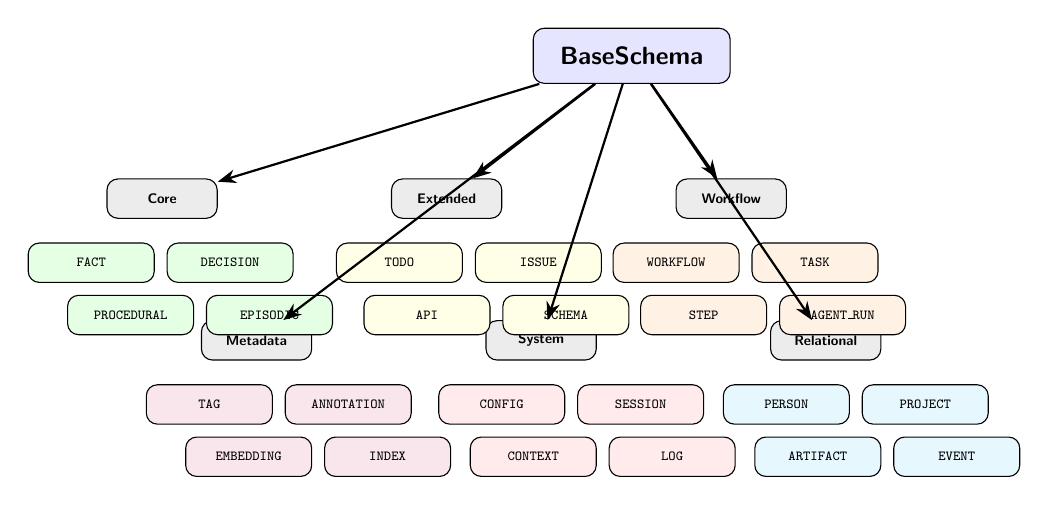
\begin{tikzpicture}[
  node distance=0.6cm and 0.4cm,
  base/.style={draw, rounded corners, font=\small\bfseries\sffamily, fill=blue!10, minimum width=2.5cm, minimum height=0.7cm},
  cat/.style={draw, rounded corners, font=\tiny\bfseries\sffamily, fill=gray!15, minimum width=1.4cm, minimum height=0.5cm},
  typ/.style={draw, rounded corners, font=\tiny\ttfamily, minimum width=1.6cm, minimum height=0.5cm},
  core/.style={typ, fill=green!10},
  ext/.style={typ, fill=yellow!10},
  wf/.style={typ, fill=orange!10},
  meta/.style={typ, fill=purple!10},
  sys/.style={typ, fill=red!8},
  rel/.style={typ, fill=cyan!10},
]
  \node[base] (base) {BaseSchema};

  % Subcategory labels
  \node[cat, below left=1.2cm and 4cm of base] (cl) {Core};
  \node[cat, right=2.2cm of cl] (el) {Extended};
  \node[cat, right=2.2cm of el] (wfl) {Workflow};
  \node[cat, below left=1.2cm and 2.8cm of base, yshift=-1.8cm] (ml) {Metadata};
  \node[cat, right=2.2cm of ml] (sl) {System};
  \node[cat, right=2.2cm of sl] (rl) {Relational};

  % Core types
  \node[core, below=0.3cm of cl, xshift=-0.9cm] (fact) {FACT};
  \node[core, right=0.15cm of fact] (dec) {DECISION};
  \node[core, below=0.15cm of fact, xshift=0.5cm] (proc) {PROCEDURAL};
  \node[core, right=0.15cm of proc] (ep) {EPISODIC};

  % Extended types
  \node[ext, below=0.3cm of el, xshift=-0.6cm] (todo) {TODO};
  \node[ext, right=0.15cm of todo] (issue) {ISSUE};
  \node[ext, below=0.15cm of todo, xshift=0.35cm] (api) {API};
  \node[ext, right=0.15cm of api] (schm) {SCHEMA};

  % Workflow types
  \node[wf, below=0.3cm of wfl, xshift=-0.7cm] (wf1) {WORKFLOW};
  \node[wf, right=0.15cm of wf1] (task) {TASK};
  \node[wf, below=0.15cm of wf1, xshift=0.35cm] (step) {STEP};
  \node[wf, right=0.15cm of step] (arun) {AGENT\_RUN};

  % Metadata types
  \node[meta, below=0.3cm of ml, xshift=-0.6cm] (tag) {TAG};
  \node[meta, right=0.15cm of tag] (ann) {ANNOTATION};
  \node[meta, below=0.15cm of tag, xshift=0.5cm] (emb) {EMBEDDING};
  \node[meta, right=0.15cm of emb] (idx) {INDEX};

  % System types
  \node[sys, below=0.3cm of sl, xshift=-0.5cm] (cfg) {CONFIG};
  \node[sys, right=0.15cm of cfg] (sess) {SESSION};
  \node[sys, below=0.15cm of cfg, xshift=0.4cm] (ctx) {CONTEXT};
  \node[sys, right=0.15cm of ctx] (lg) {LOG};

  % Relational types
  \node[rel, below=0.3cm of rl, xshift=-0.5cm] (per) {PERSON};
  \node[rel, right=0.15cm of per] (prj) {PROJECT};
  \node[rel, below=0.15cm of per, xshift=0.4cm] (art) {ARTIFACT};
  \node[rel, right=0.15cm of art] (evt) {EVENT};

  % Arrows from base to subcategory labels
  \draw[-{Stealth}, thick] (base) -- (cl);
  \draw[-{Stealth}, thick] (base) -- (el);
  \draw[-{Stealth}, thick] (base) -- (wfl);
  \draw[-{Stealth}, thick] (base) -- (ml);
  \draw[-{Stealth}, thick] (base) -- (sl);
  \draw[-{Stealth}, thick] (base) -- (rl);
\end{tikzpicture}
\end{center}

\section{OTP Application Startup}\label{app:startup}

The \texttt{MemoryLayer} application module initializes ETS tables and Mnesia before starting the supervision tree:

\begin{lstlisting}[caption={Application startup: ETS and Mnesia initialization.}, label={lst:app-startup}]
defmodule MemoryLayer do
  use Application

  @impl true
  def start(_type, _args) do
    # Create ETS tables for working memory
    :ets.new(:memory_working, [
      :set, :public, :named_table,
      read_concurrency: true
    ])
    :ets.new(:memory_lru, [
      :set, :public, :named_table
    ])

    # Initialize Mnesia schema and tables
    :mnesia.create_schema([node()])
    :mnesia.start()
    :mnesia.create_table(:memories, [
      attributes: [:id, :data],
      type: :set,
      disc_copies: [node()]
    ])
    :mnesia.create_table(:versions, [
      attributes: [:id, :entry],
      type: :bag,
      disc_copies: [node()]
    ])
    :mnesia.create_table(:edges, [
      attributes: [:key, :edge],
      type: :bag,
      disc_copies: [node()]
    ])

    # Start supervision tree
    children = [
      MemoryLayer.Schema.Registry,
      MemoryLayer.Graph,
      MemoryLayer.Storage
    ]

    opts = [
      strategy: :one_for_one,
      name: MemoryLayer.Supervisor
    ]
    Supervisor.start_link(children, opts)
  end
end
\end{lstlisting}

The \texttt{:one\_for\_one} supervision strategy restarts individual processes independently: if the Graph GenServer crashes, the Schema Registry and Storage continue running unaffected.

\section{Mix Project Configuration}\label{app:mix}

The project dependencies are minimal, leveraging OTP's built-in capabilities:

\begin{lstlisting}[caption={mix.exs: project configuration.}, label={lst:mix}]
defmodule MemoryLayer.MixProject do
  use Mix.Project

  def project do
    [
      app: :memory_layer,
      version: "0.1.0",
      elixir: "~> 1.16",
      start_permanent: Mix.env() == :prod,
      deps: deps()
    ]
  end

  def application do
    [
      extra_applications: [:logger, :mnesia, :crypto],
      mod: {MemoryLayer, []}
    ]
  end

  defp deps do
    [
      {:uuid, "~> 1.1"},
      {:jason, "~> 1.4"},
      {:ex_doc, "~> 0.31", only: :dev, runtime: false},
      {:dialyxir, "~> 1.4", only: [:dev, :test],
        runtime: false}
    ]
  end
end
\end{lstlisting}

The only runtime dependencies beyond OTP are \texttt{uuid} (for generating memory identifiers) and \texttt{jason} (for JSON serialization in the MCP interface).
ETS, Mnesia, and \texttt{:crypto} are all built-in OTP applications.

\section{Version Chain Diagram}\label{app:version-chain}

A typical memory evolution chain with change reasons:

\begin{center}
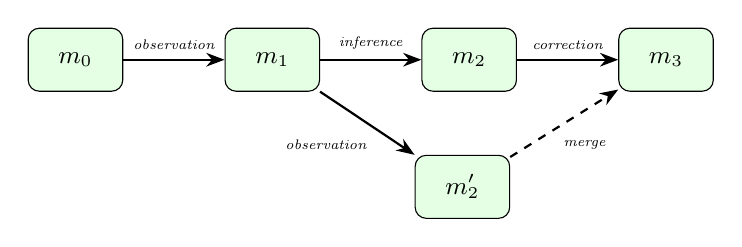
\begin{tikzpicture}[
  node distance=2.5cm,
  mem/.style={draw, rounded corners, fill=green!10, minimum width=1.2cm, minimum height=0.8cm, font=\small},
  arr/.style={-{Stealth}, thick},
  lab/.style={font=\tiny\itshape, above, midway}
]
  \node[mem] (m0) {$m_0$};
  \node[mem, right of=m0] (m1) {$m_1$};
  \node[mem, right of=m1] (m2) {$m_2$};
  \node[mem, right of=m2] (m3) {$m_3$};
  \node[mem, below right=0.8cm and 1.2cm of m1] (m2p) {$m_2'$};

  \draw[arr] (m0) -- node[lab] {observation} (m1);
  \draw[arr] (m1) -- node[lab] {inference} (m2);
  \draw[arr] (m2) -- node[lab] {correction} (m3);
  \draw[arr, dashed] (m2p) -- node[lab, below right, pos=0.4] {merge} (m3);
  \draw[arr] (m1) -- node[lab, below left, pos=0.6] {observation} (m2p);
\end{tikzpicture}
\end{center}

In this example, $m_0$ is created via observation, then $m_1$ is inferred from it.
A concurrent modification produces $m_2$ and $m_2'$.
The conflict is resolved by merging into $m_3$ with a correction reason.

\end{document}
